\casesection{Two-dimensional radial free surface oscillations \label{case:thacker2d}}


\paragraph*{Purpose}
In the test case \emph{One-dimensional planar free surface oscillations}, the key phenomena of flooding and drying are investigated for a one-dimensional model. In the present test case, a two-dimensional case is investigated. In the two-dimensional case, free surface oscillations will be considered for a radially symmetric case with a curved free surface. An analytical solution is available to compare the numerical results with (William Thacker, \emph{Some exact solutions to the nonlinear shallow-water wave equations}, J. Fluid Mech. (1981), vol. 107, pp. 499-608).



\paragraph*{Linked claims}
Claims that are related to the current test case are:
\begin{itemize}
\item \clrefnoh{cl:generalGrids}
\item \clrefnoh{cl:advectionShortwave}
\item \clrefnoh{cl:advectionFloodingdrying}
\end{itemize}

\paragraph*{Approach}
A test model setup is set up to match with the assumptions associated with the analytical solution. The setup yields a paraboloid topography, prescribed as:
\begin{equation*}
z(r)  =  -D_0 \left(1 - \frac{r^2}{a^2}  \right)
\end{equation*}
with $-D_0$ the lowest bed level of the geometry and $a$ a measure for the steepness of the bed. Thacker has figured out multiple analytical solutions for two-dimensional cases in the absence of bed friction. One of them comprises the description of oscillations for which the surface is curved. Three grids are generated to represent the paraboloid on: a grid containing hexagon cells, a grid containing square cells and a grid containing triangular cells (shown in \Fref{fig:thacker2dgrids}).

\begin{figure}[h!]
\begin{center}
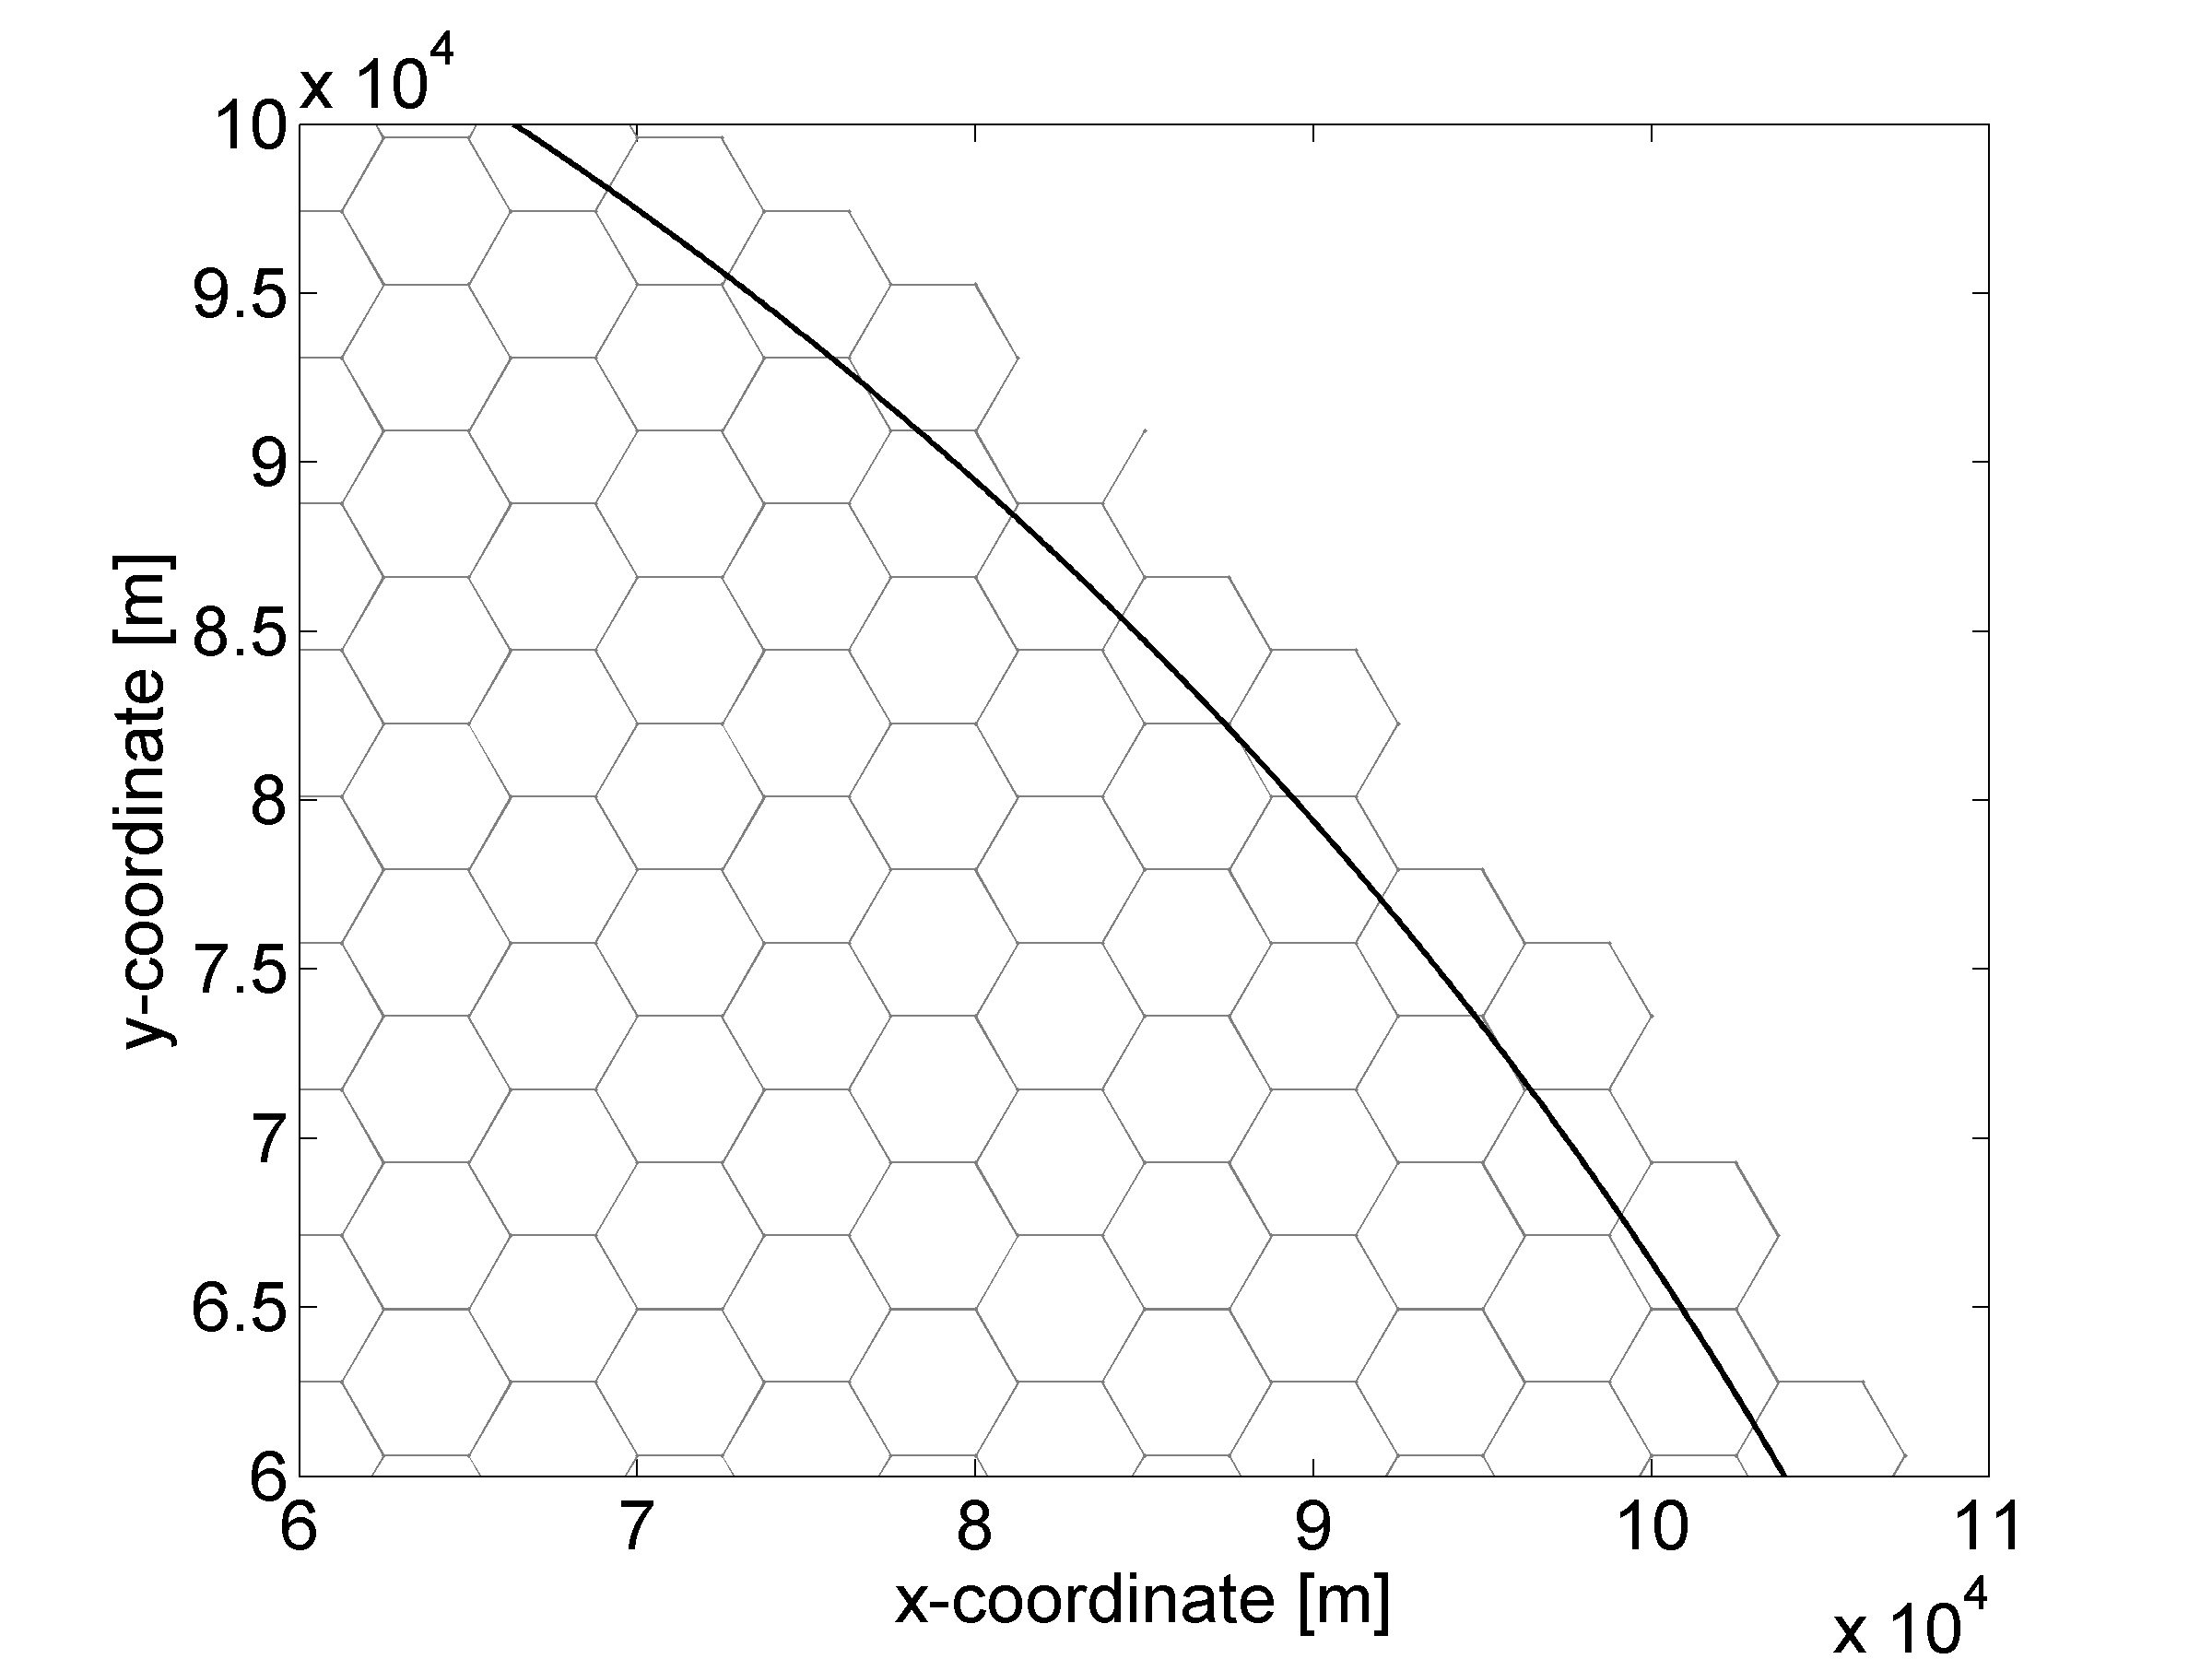
\includegraphics[width=0.32\columnwidth]{../../c043_thacker2d_hexagons/doc/figures/thacker2dgridhexagons.png}
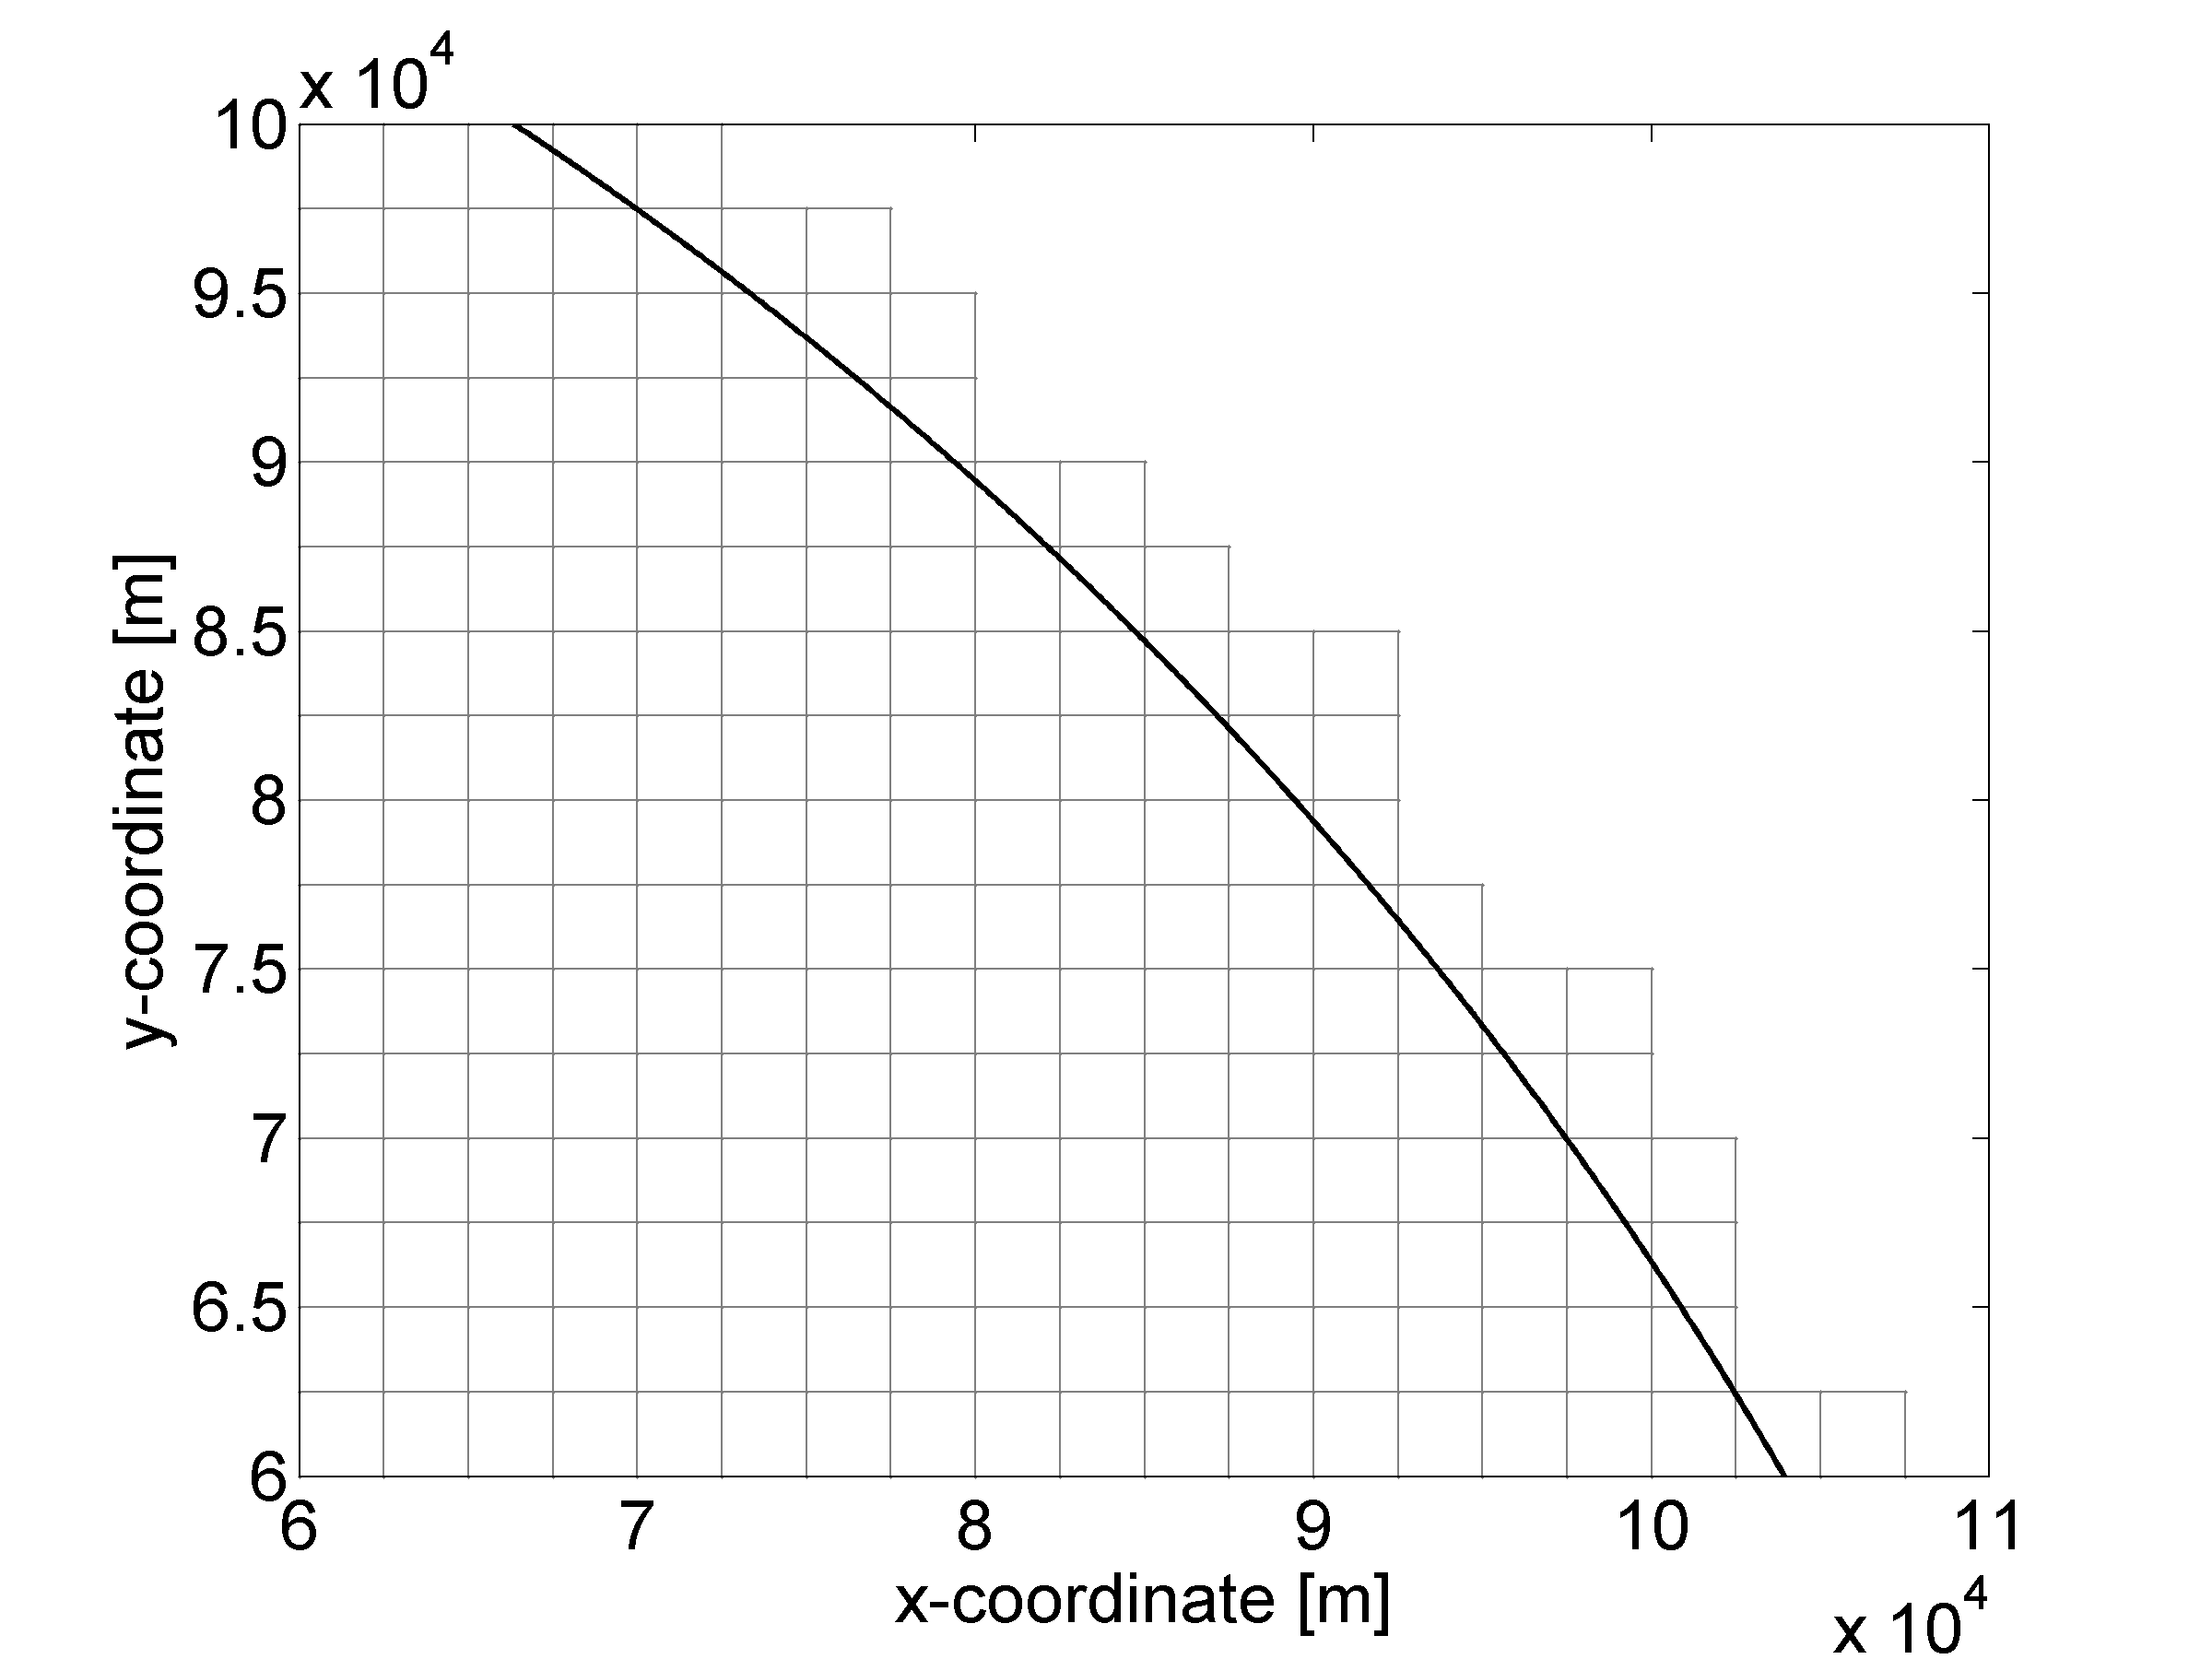
\includegraphics[width=0.32\columnwidth]{../../c044_thacker2d_squares/doc/figures/thacker2dgridsquares.png}
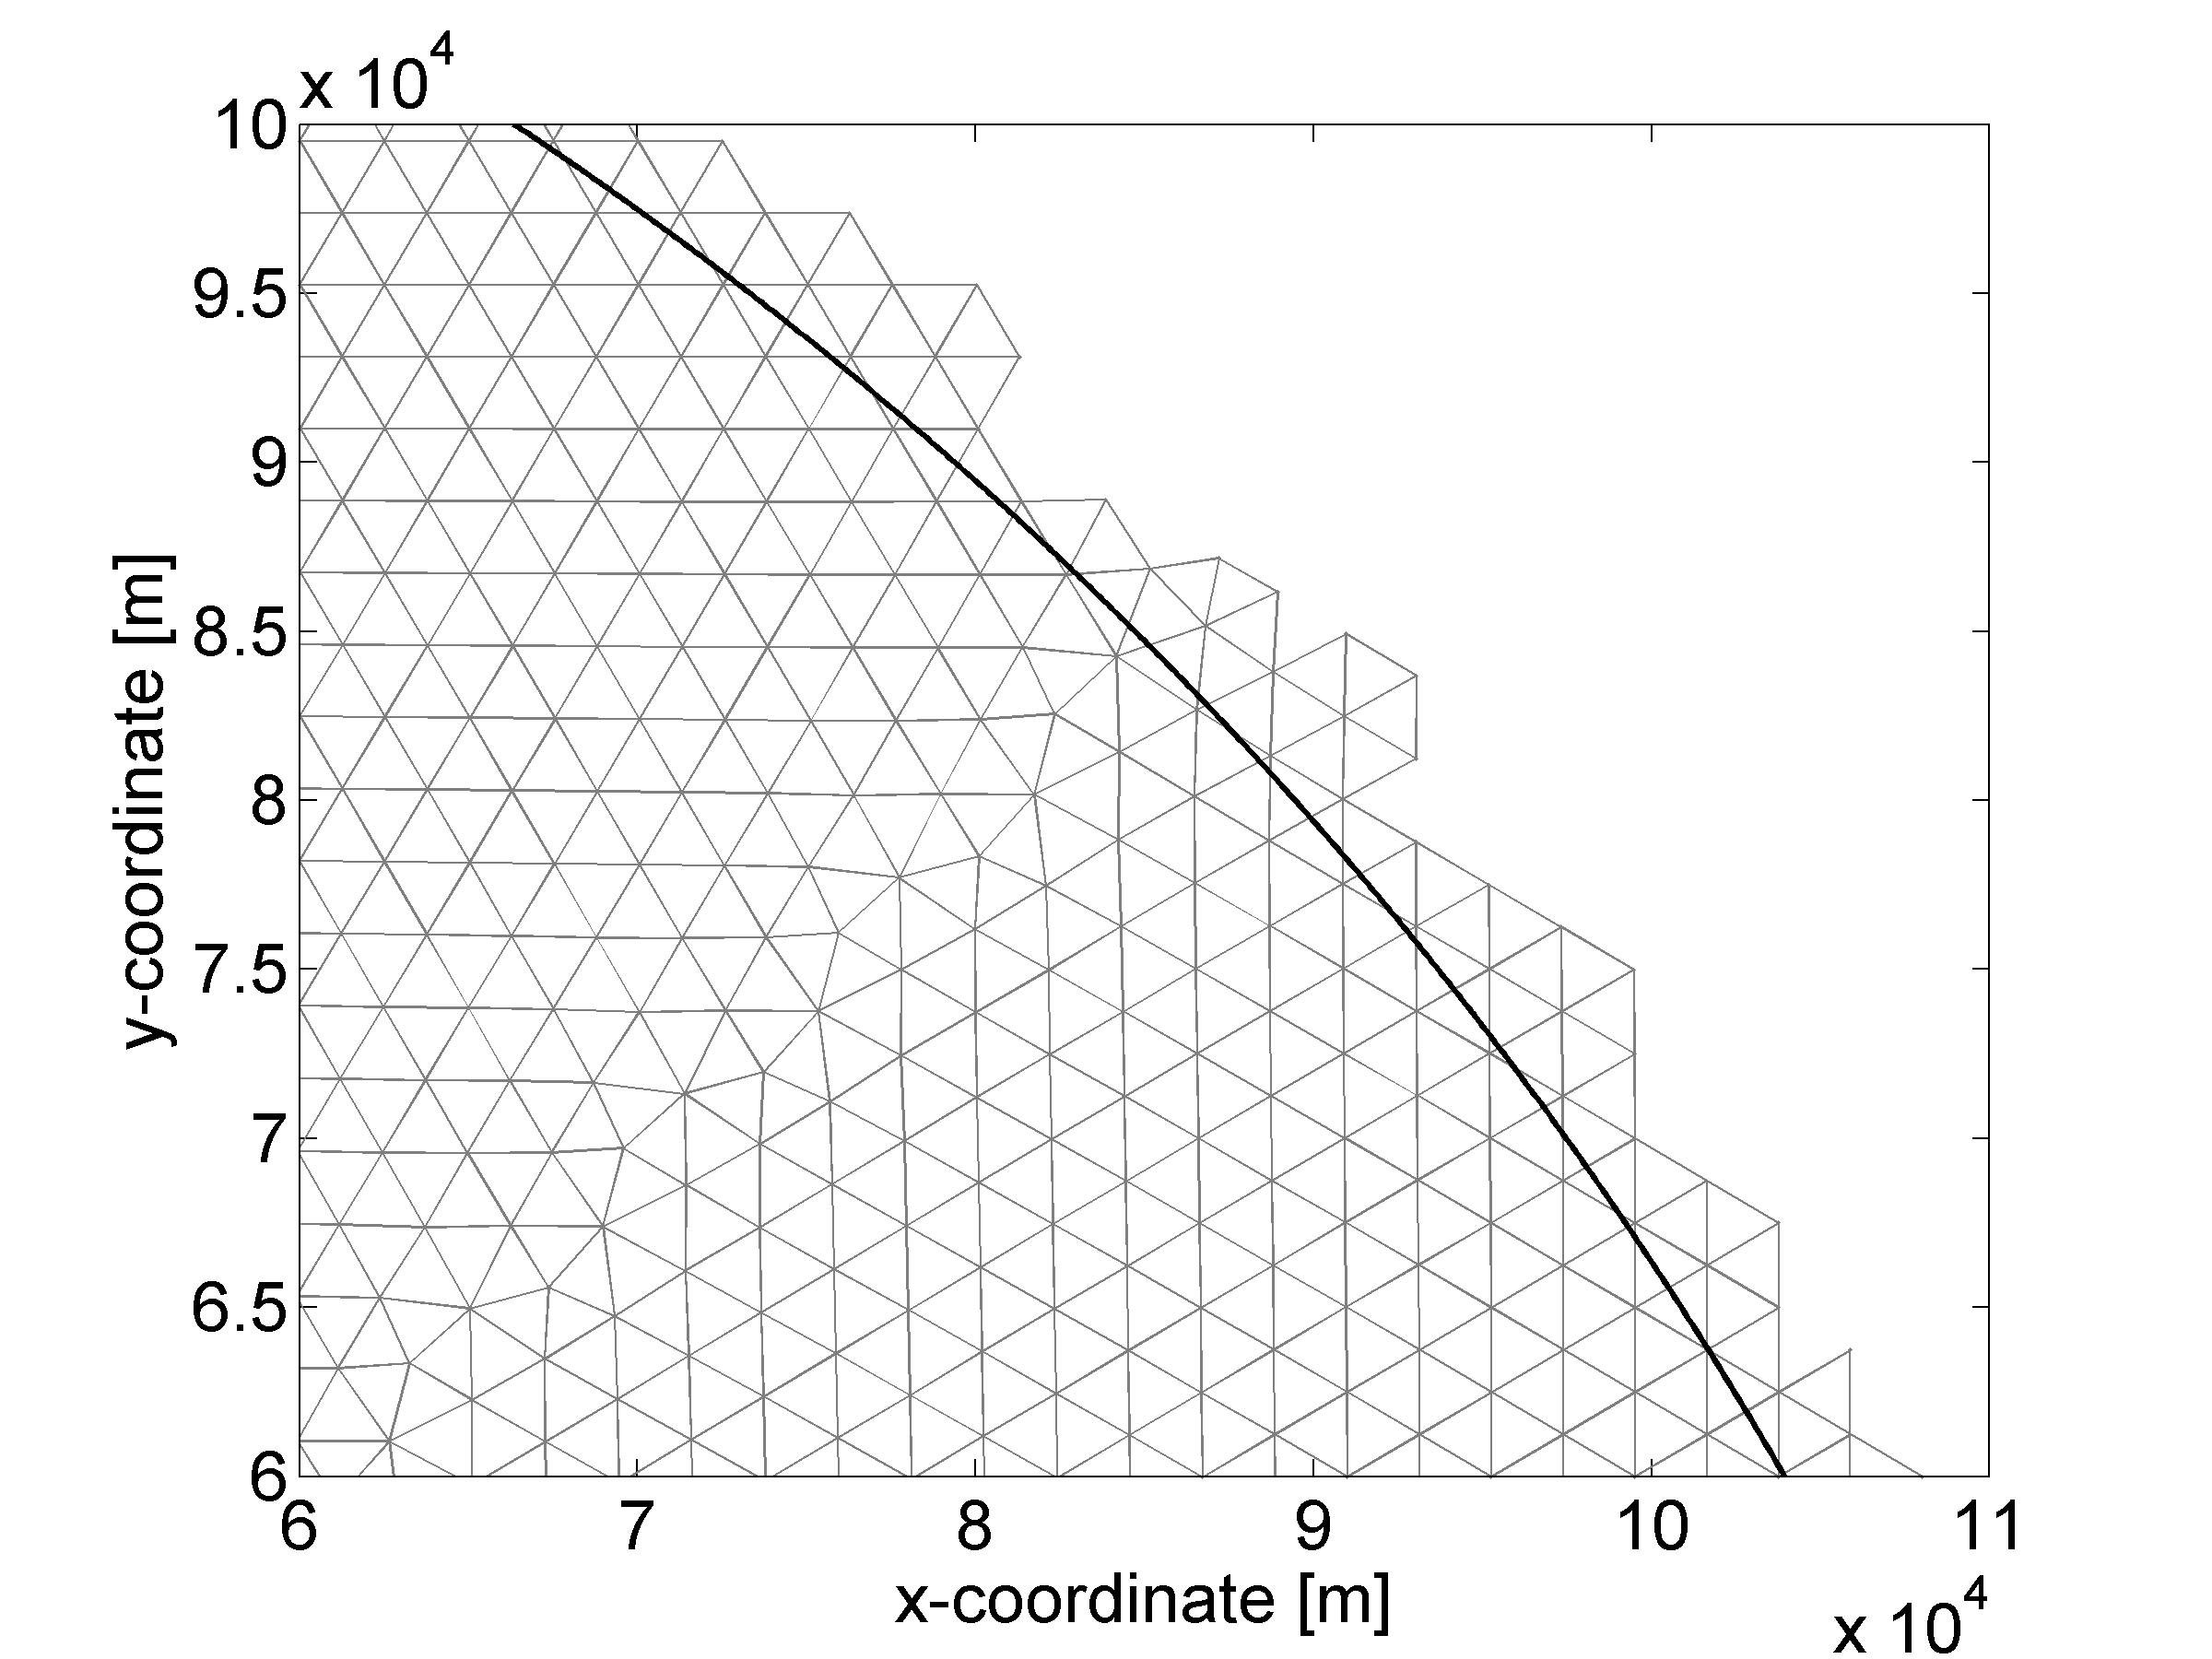
\includegraphics[width=0.32\columnwidth]{../../c045_thacker2d_triangles/doc/figures/thacker2dgridtriangles.png}
\end{center}\caption{Computational grids for the testcase (only a detail is shown). From left to right: grid with hexagon cells, square cells and triangular cells. The curved black line marks the circular area of interest (radius $R = 120$~km). Notice that the grids become finer from left to right. \label{fig:thacker2dgrids}}
\end{figure}

The analytical solution comprises a curved free surface and an initial zero-velocity field. The solution, derived by Thacker, describes the water level and velocity magnitude as a function of the radius $r$ and the time $t$. Although acceleration due to Coriolis' forces are present in the solution, the Coriolis' effect is disregarded in the present test case. Without the Coriolis' effect, the solution reads:
\begin{eqnarray*}
h(r,t)  &=& D_0 \left\{ \frac{\sqrt{1-A^2}}{1-A \cos \omega t} - 1 - \frac{r^2}{L^2} \left[ \frac{1-A^2}{\left(1-A \cos \omega t  \right)^2} - 1  \right]  \right\}   \\
u(r,t)  &=&  \frac{1}{2} r \omega  \left| \frac{ A \sin \omega t}{1-A \cos \omega t }  \right|
\end{eqnarray*}
for the water level $h$ and the velocity magnitude $u$ in which:
\begin{eqnarray*}
A  &=&  \frac{(D_0 + \eta)^2 - D_0^2}{(D_0 + \eta)^2 + D_0^2}  \\
\omega^2  &=&  \frac{8 g D_0}{L^2}
\end{eqnarray*}
in which $L = a = 102$~km (geometry of the paraboloid), $D_0 = 10$~m (distance from deepest point to the reference level) and $\eta = 2$~m the largest positive surface elevation (w.r.t.\ the reference level). The parameter $g = 9.81$~m/s$^2$ represents the gravitation acceleration.



\paragraph*{Model description}
The used grids are (partially) shown in \Fref{fig:thacker2dgrids}. Friction and diffusion are switched off. As already mentioned, the following parameter values are used: $L = a = 102$~km, $D_0 = 10$~m and $\eta = 2$~m. Hence, via $\omega$, one period $T = 2 \pi / \omega = 22877$~s $\approx 6.35$~hours. The run time yields two periodic cycles. Advection scheme \texttt{33} is used. The parameter \texttt{chkadvd = 0}.



\paragraph*{Results}
The final result for the grid containing hexagons is provided in \Fref{fig:thacker2dhexagonsT2}. 

\begin{figure}[h!]
\begin{center}
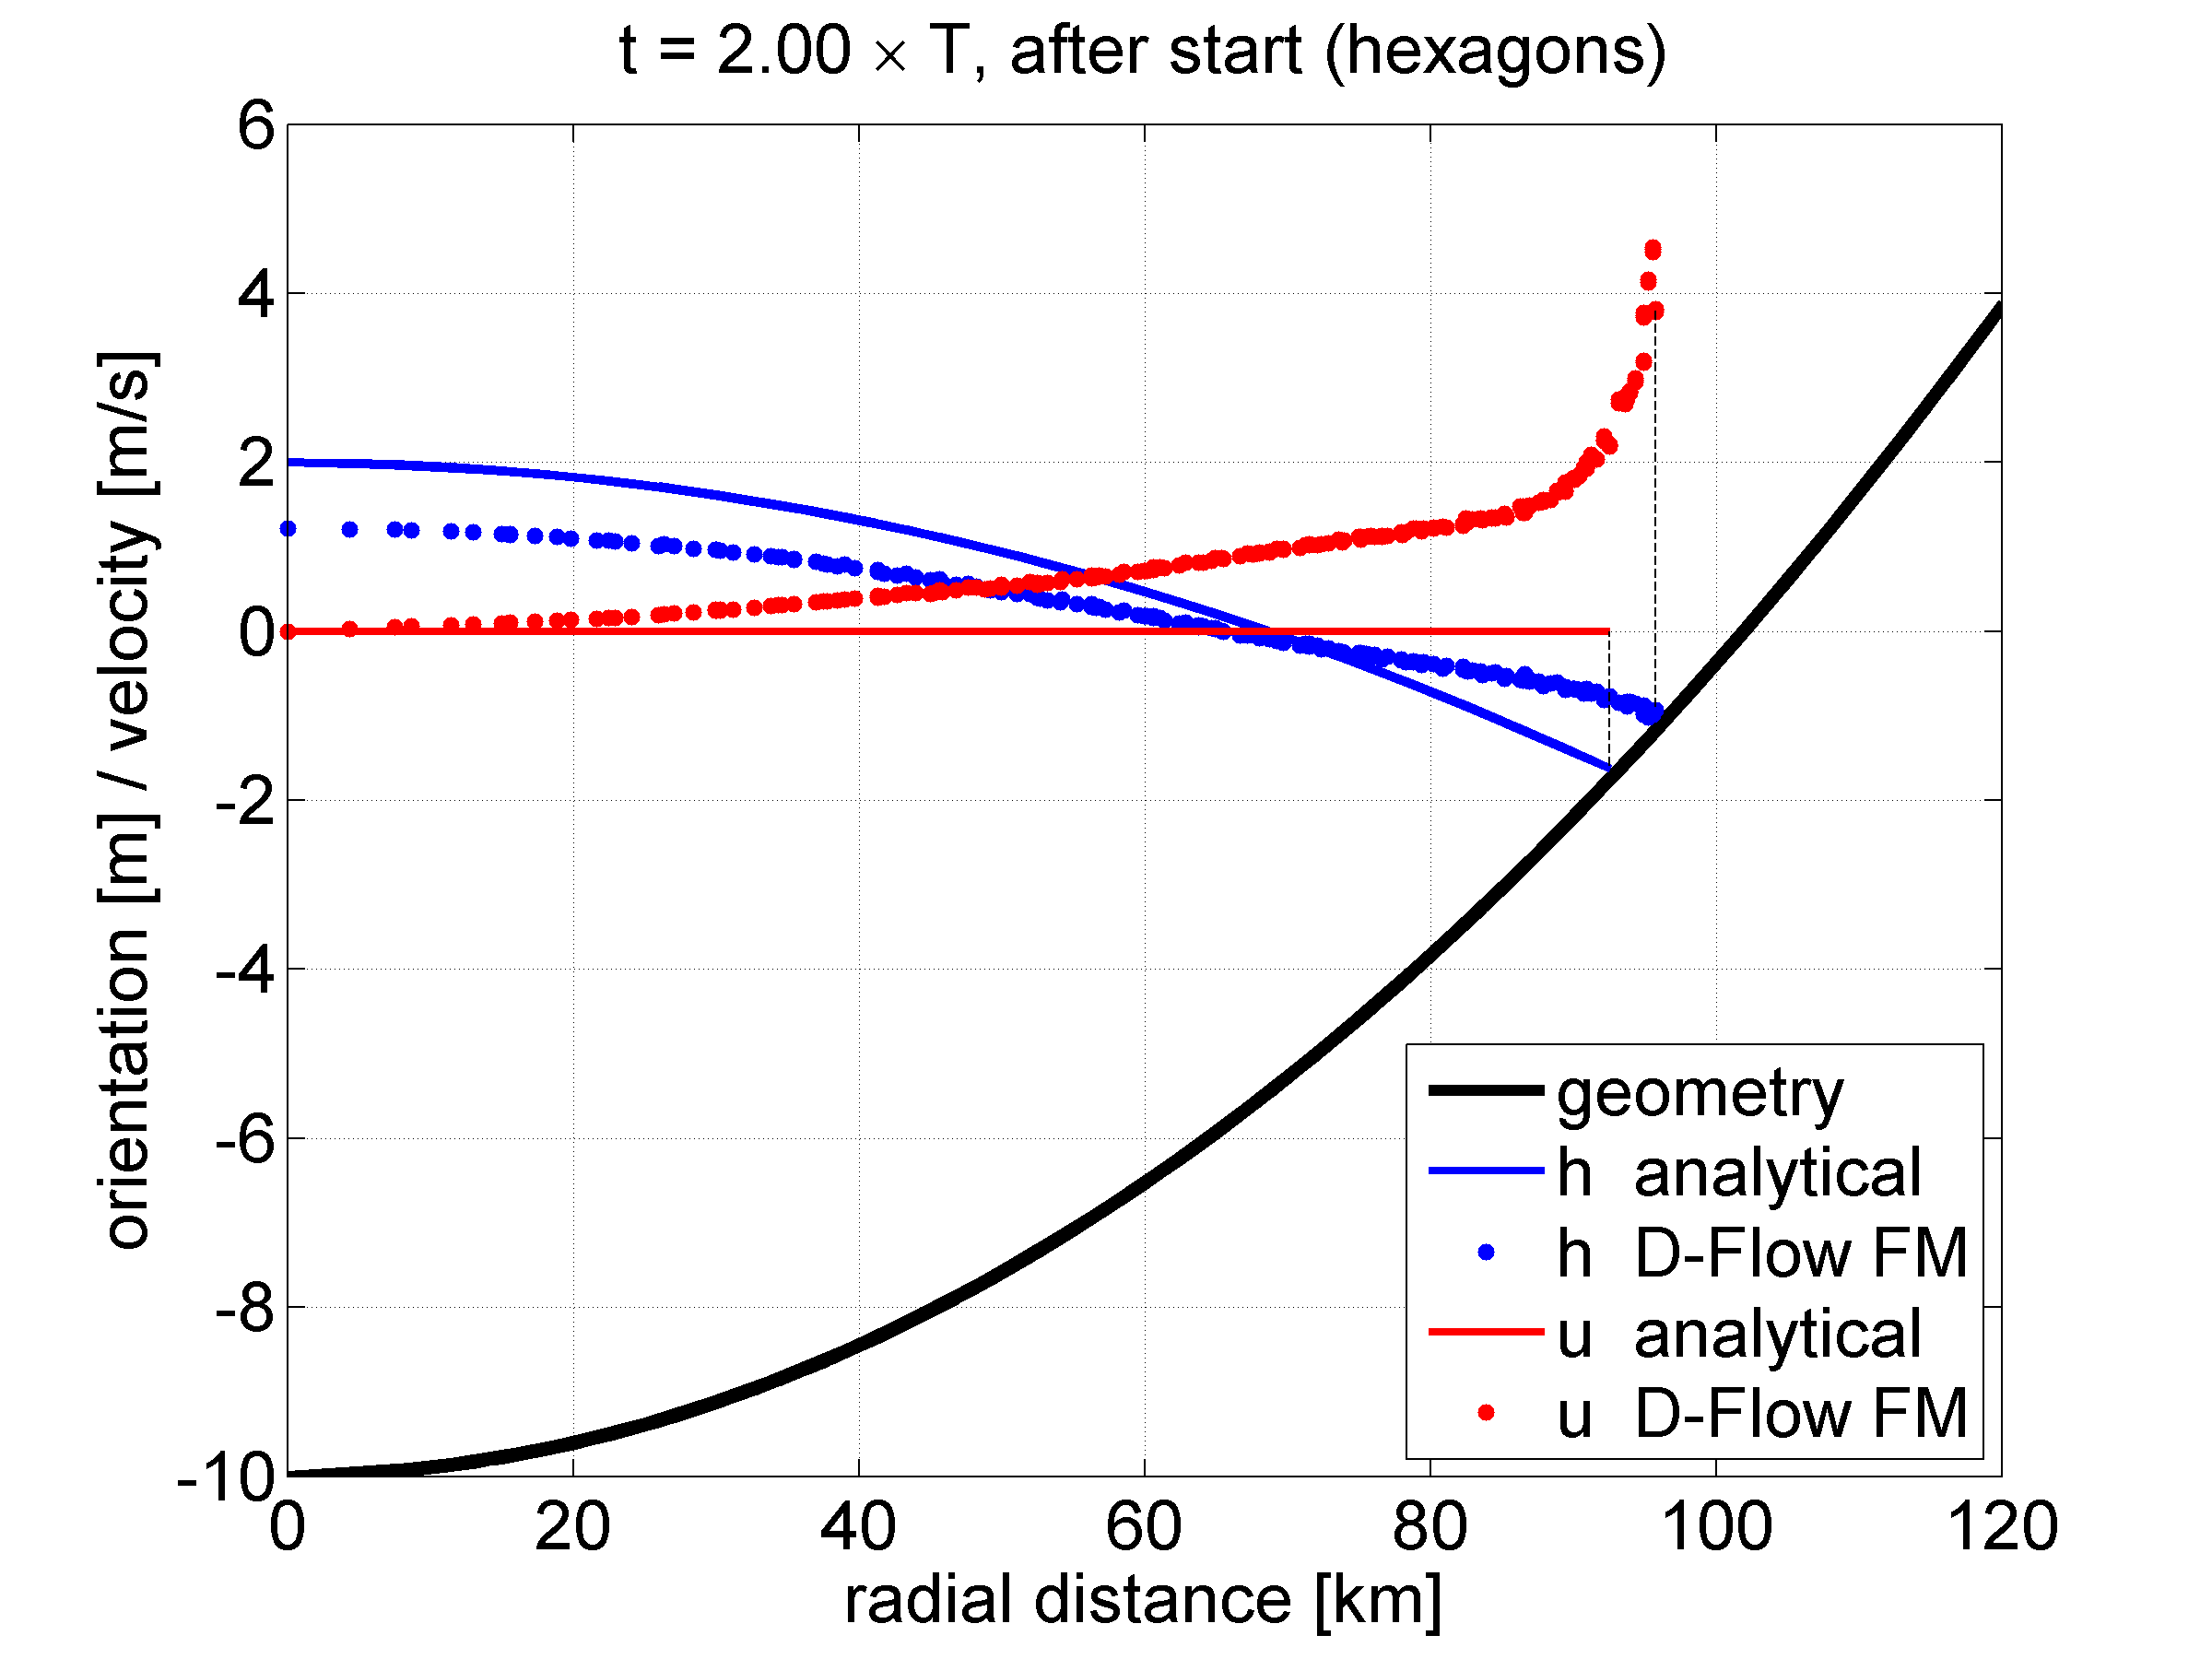
\includegraphics[width=0.57\columnwidth]{../../c043_thacker2d_hexagons/doc/figures/thacker2dhexagonsT2.png}
\end{center}\caption{Computational results for the testcase on the hexagonal grid. The values on the vertical axis represent water levels [m w.r.t.\ reference] related to the data represented in blue and represent velocities [m/s] related to the data represented in red. \label{fig:thacker2dhexagonsT2}}
\end{figure}

This figure shows the analytical and numerical solutions for $h$ (in blue) and $u$ (in red) at $t = 2T$. The computational results are projected onto the one axis of symmetry. The point at which the blue graphs and black parabola intersect can be perceived as the shoreline. The difference between the locations of the shoreline from the analytical and numerical solution is marked by two vertical black dashed lines. Analagous figures are shown in \Fref{fig:thacker2dresults} for all the three grids (varying from top to bottom) and two points in time: $t = T$ (left panels) and $t = 2T$ (right panels).

\begin{figure}[h!]
\begin{center}
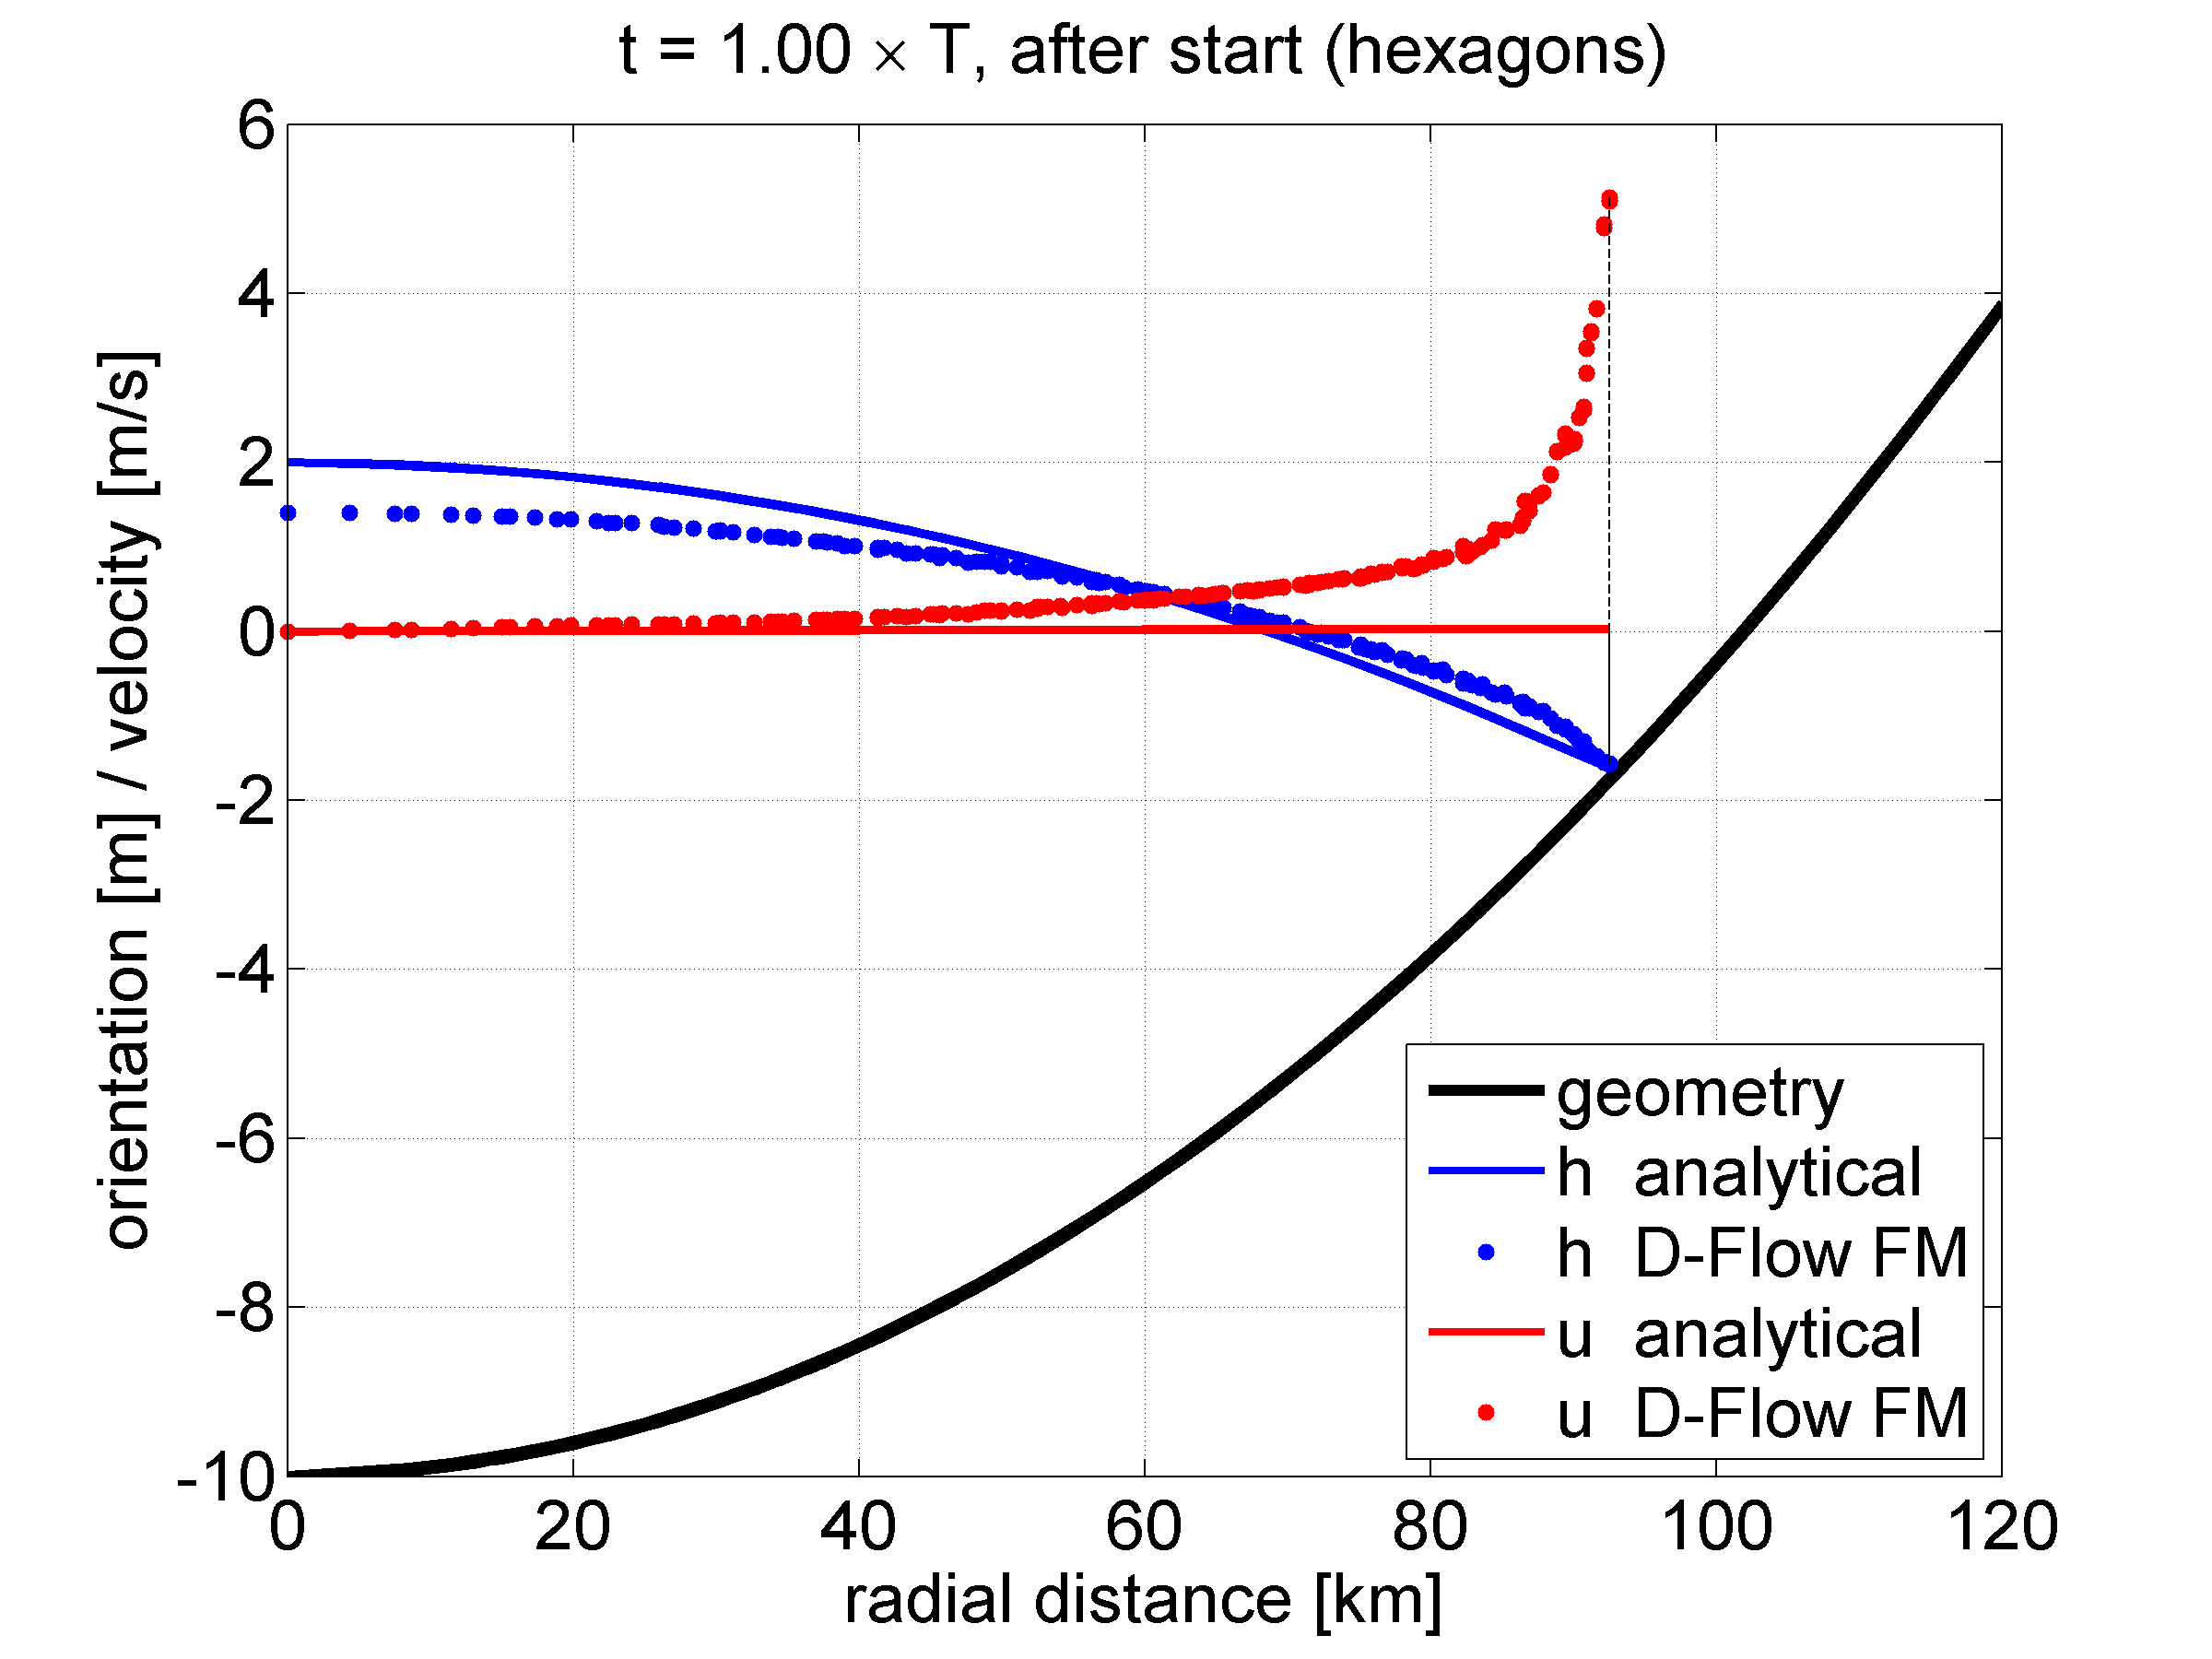
\includegraphics[width=0.48\columnwidth]{../../c043_thacker2d_hexagons/doc/figures/thacker2dhexagonsT1.png}
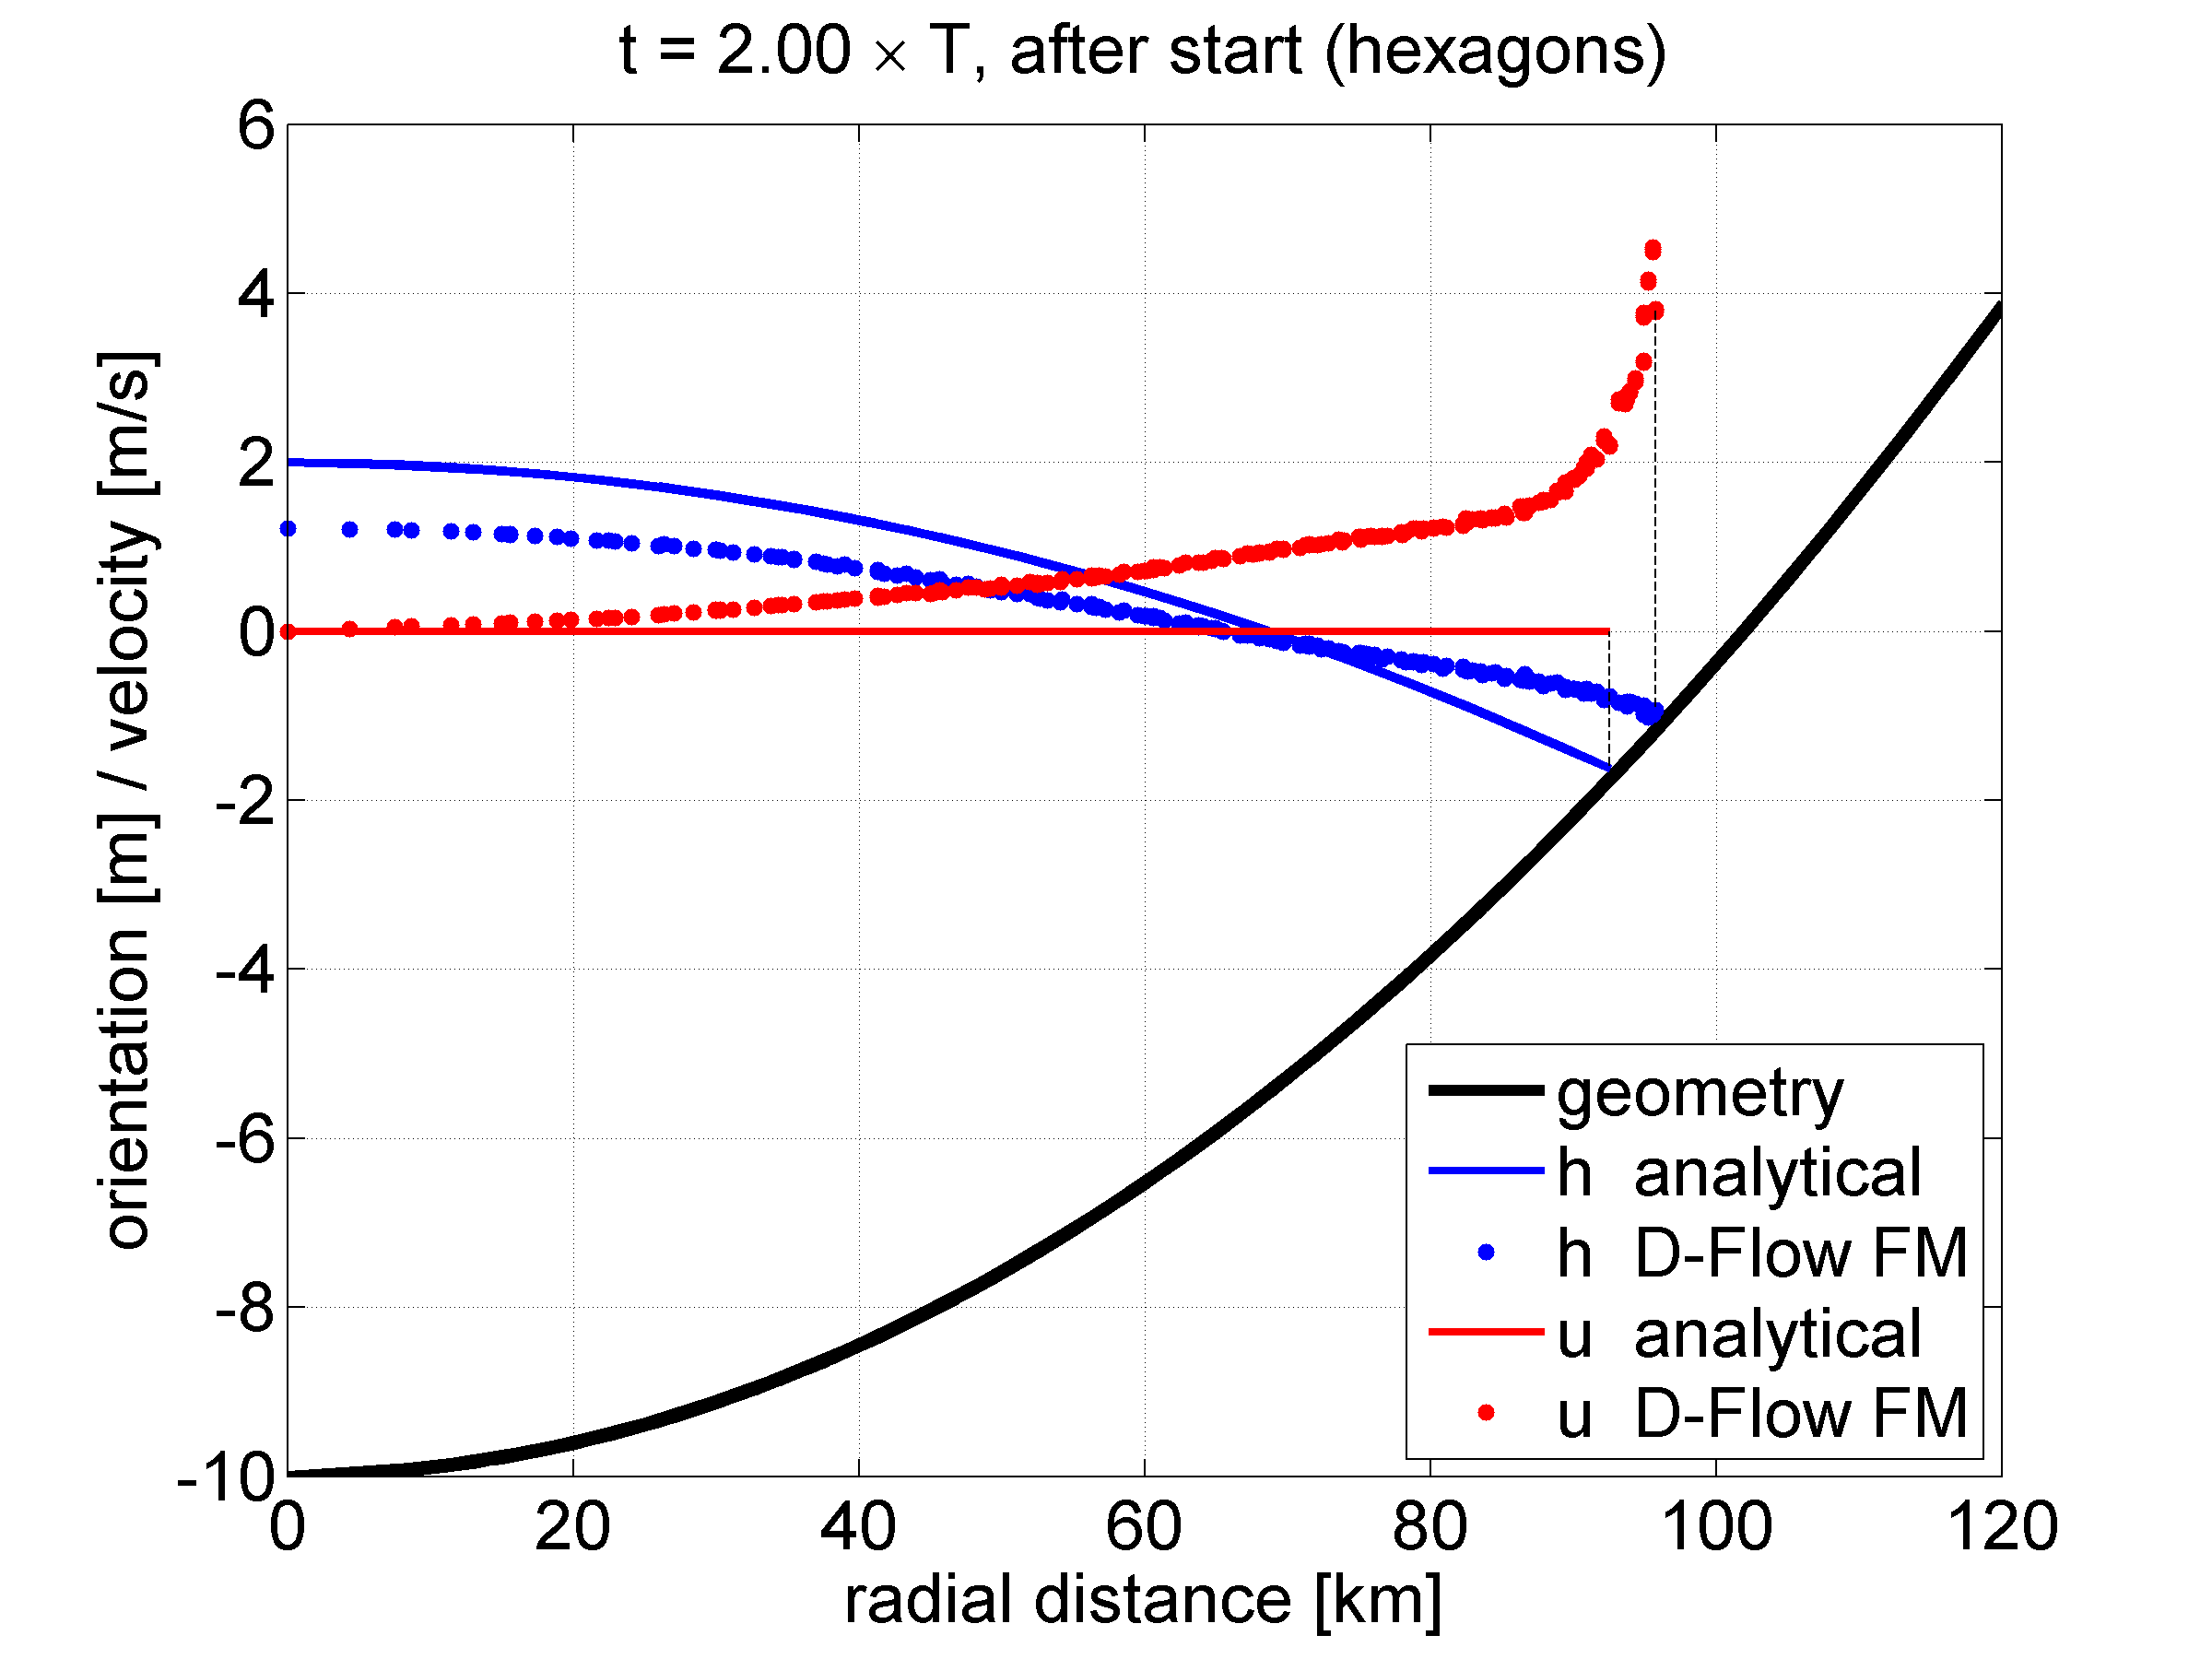
\includegraphics[width=0.48\columnwidth]{../../c043_thacker2d_hexagons/doc/figures/thacker2dhexagonsT2.png} \\
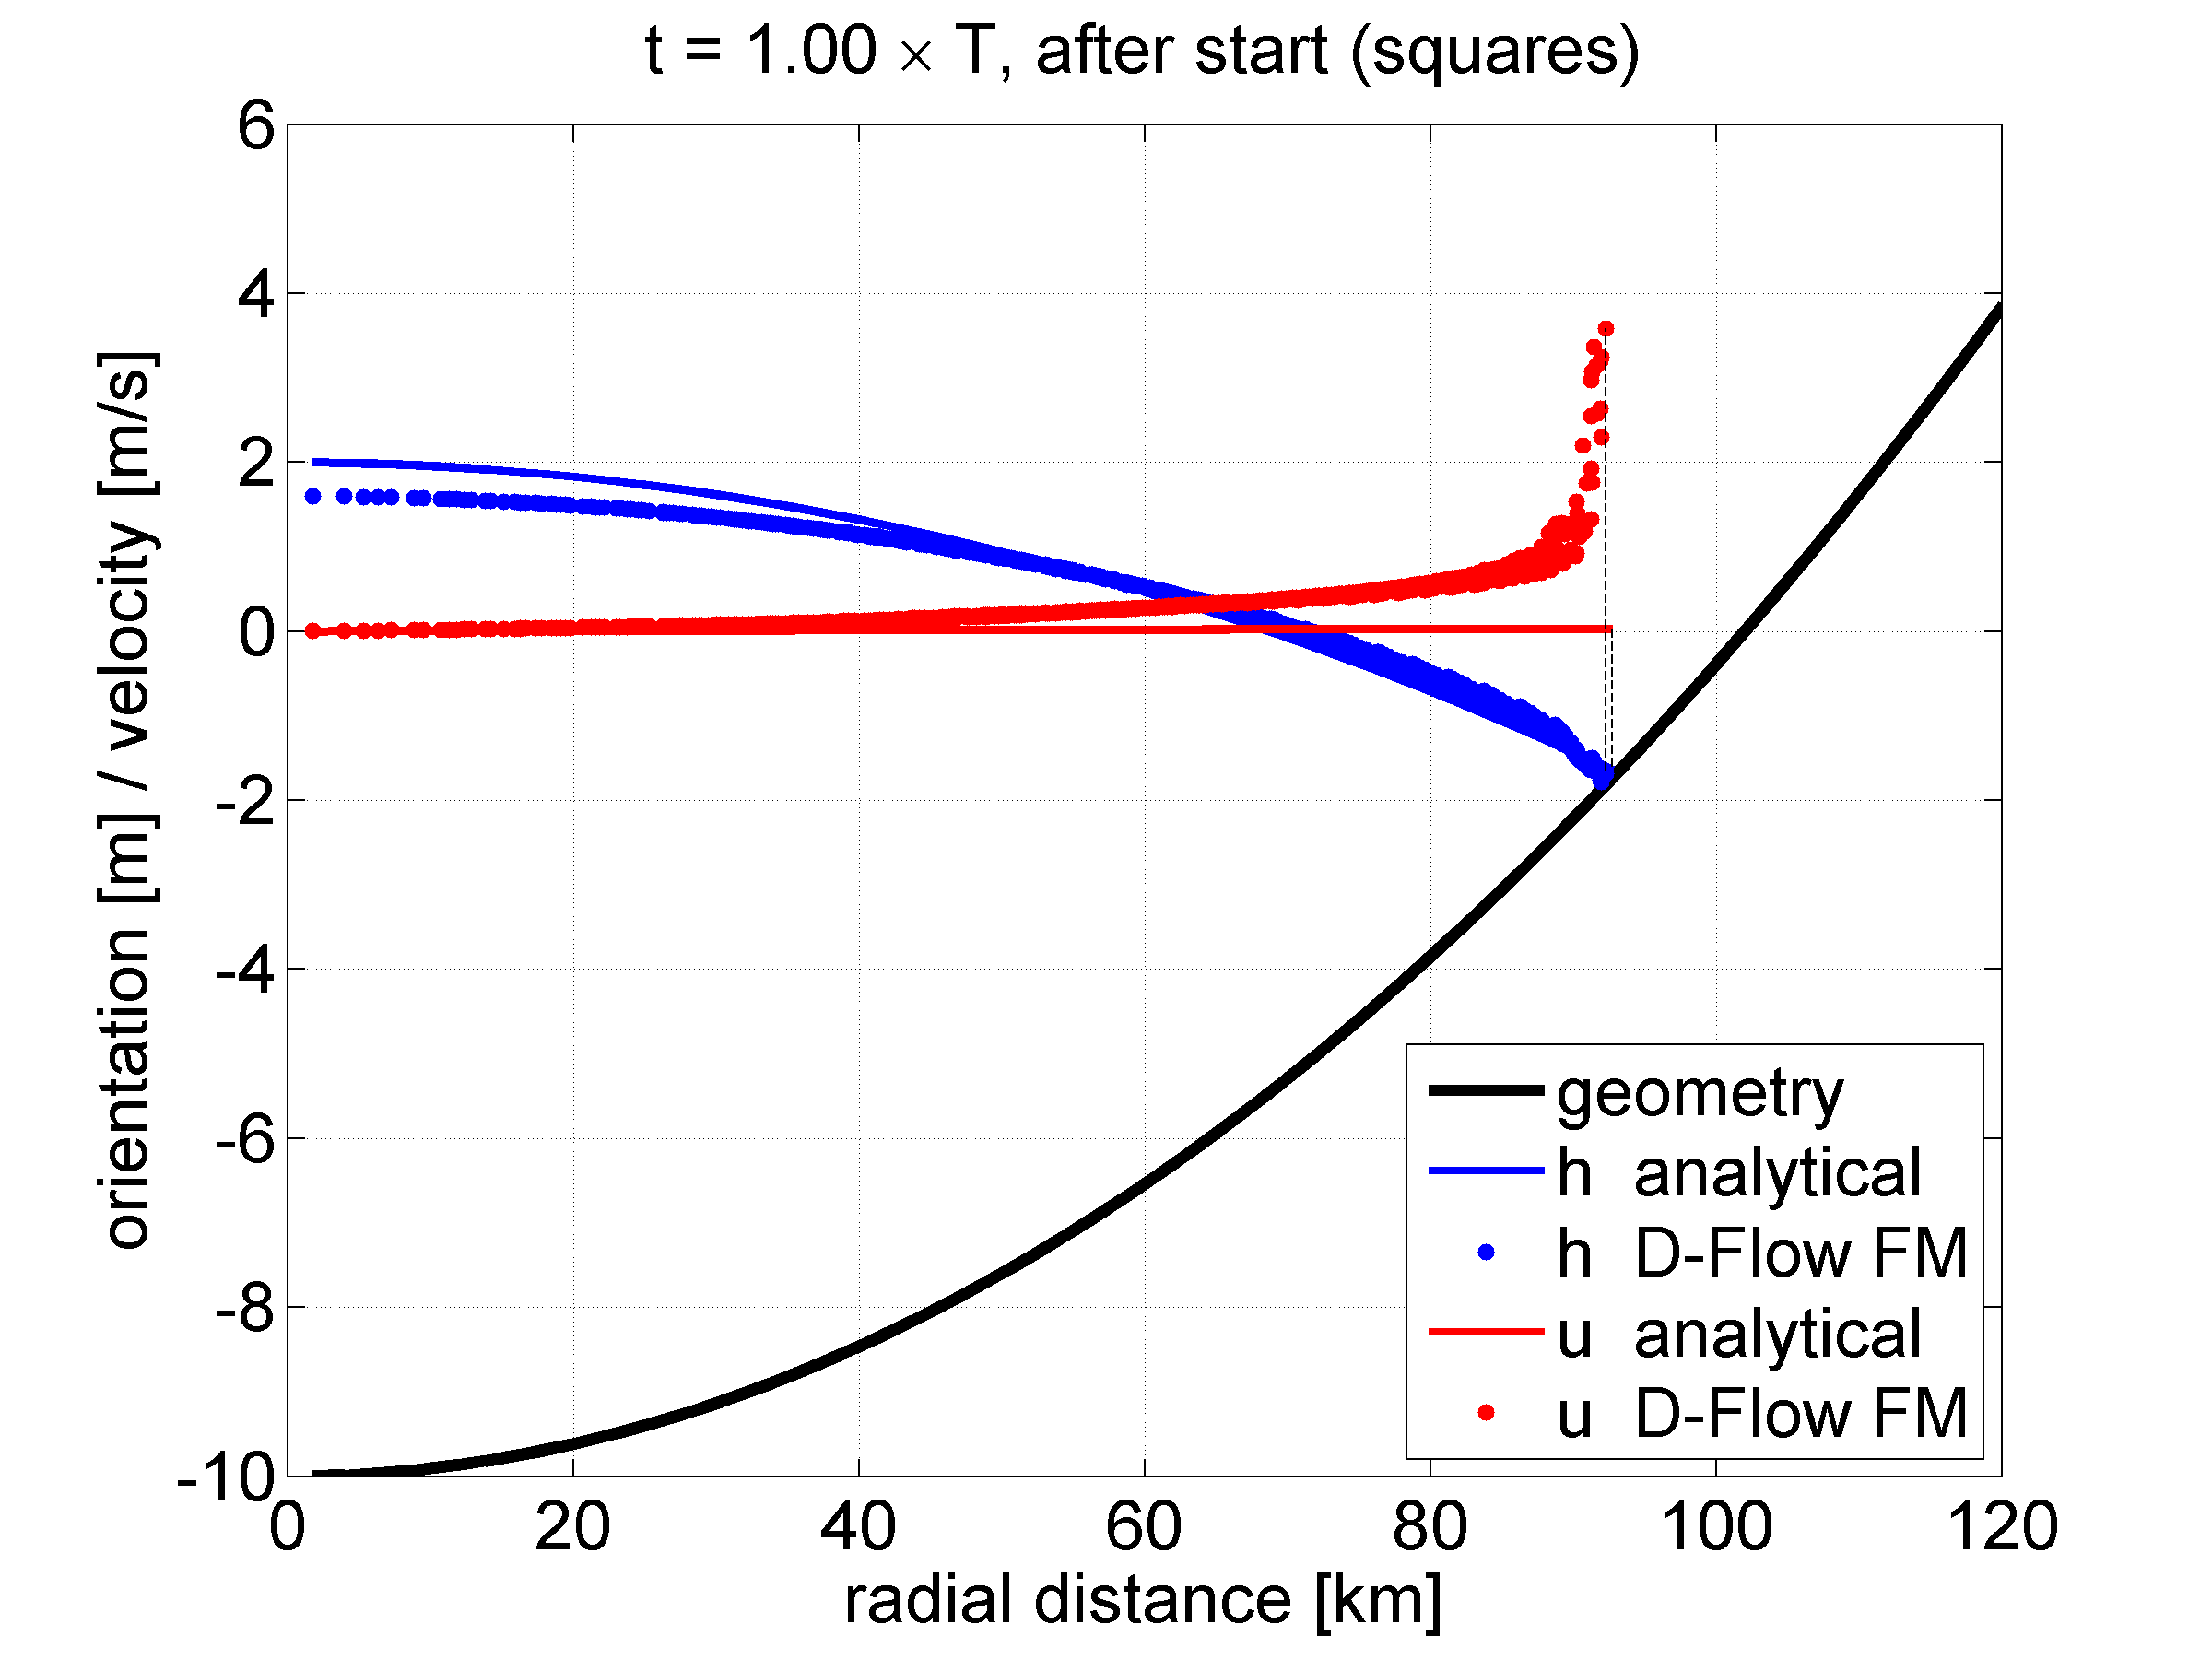
\includegraphics[width=0.48\columnwidth]{../../c044_thacker2d_squares/doc/figures/thacker2dsquaresT1.png}
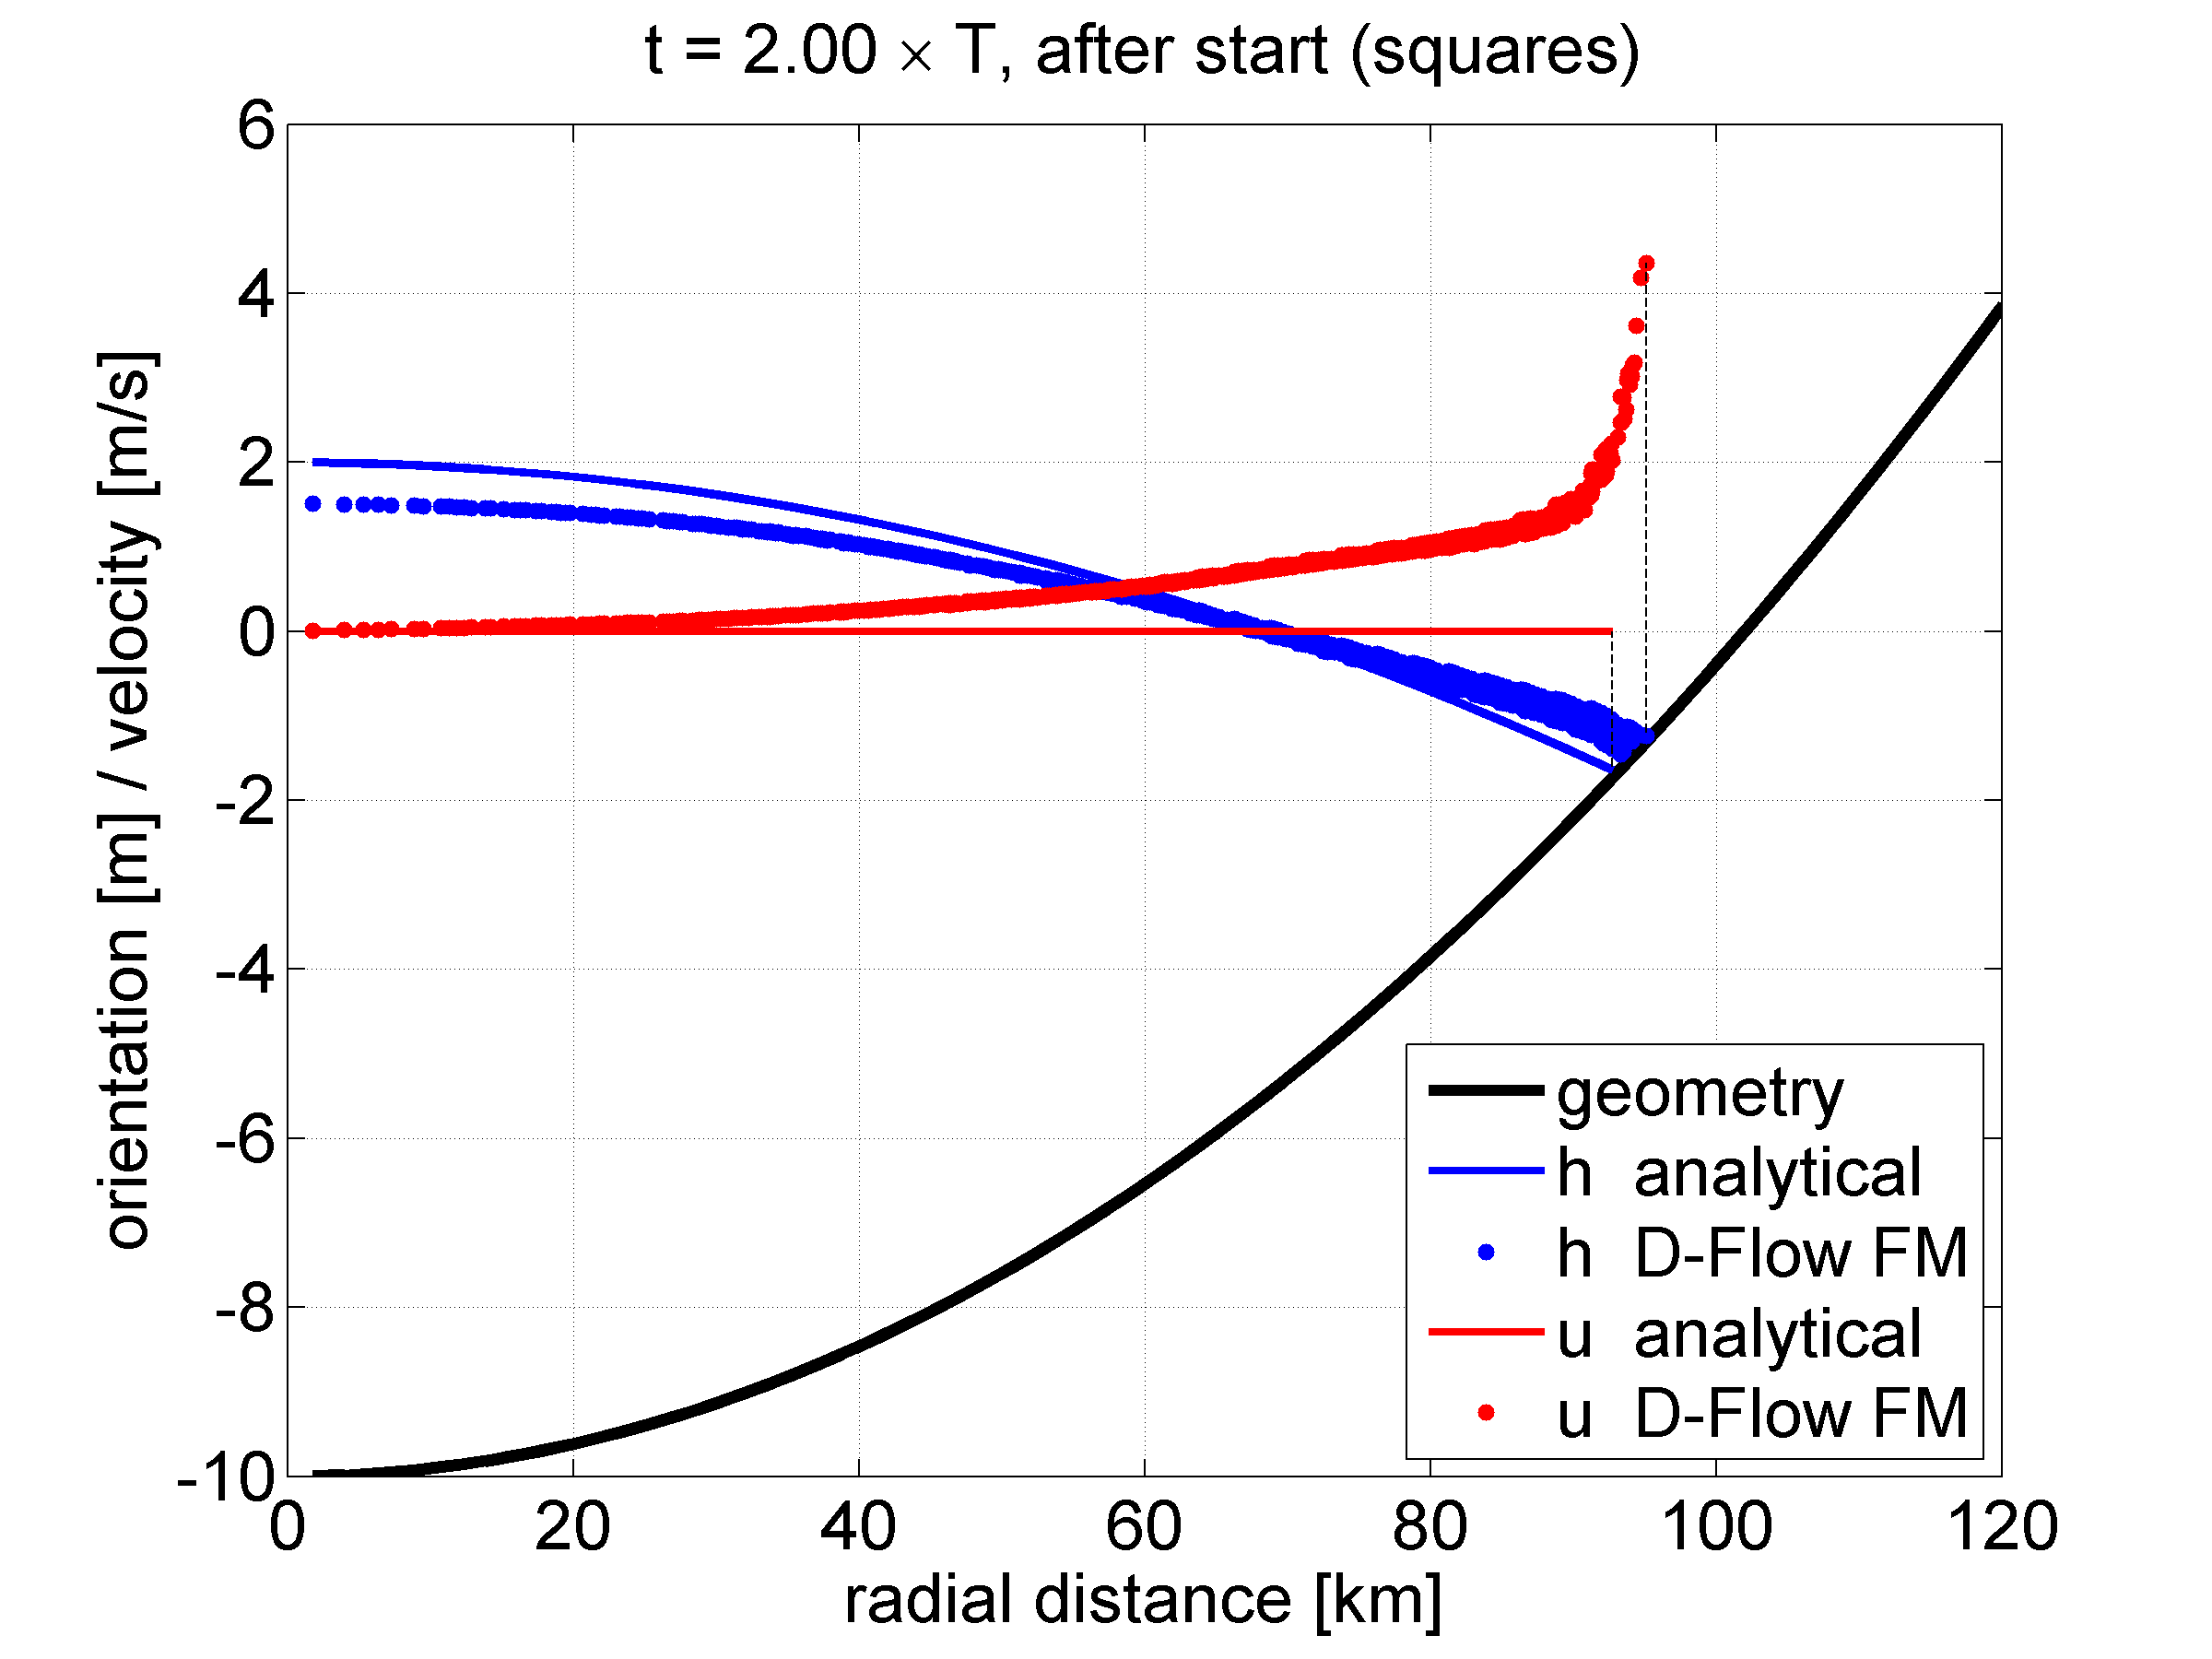
\includegraphics[width=0.48\columnwidth]{../../c044_thacker2d_squares/doc/figures/thacker2dsquaresT2.png} \\
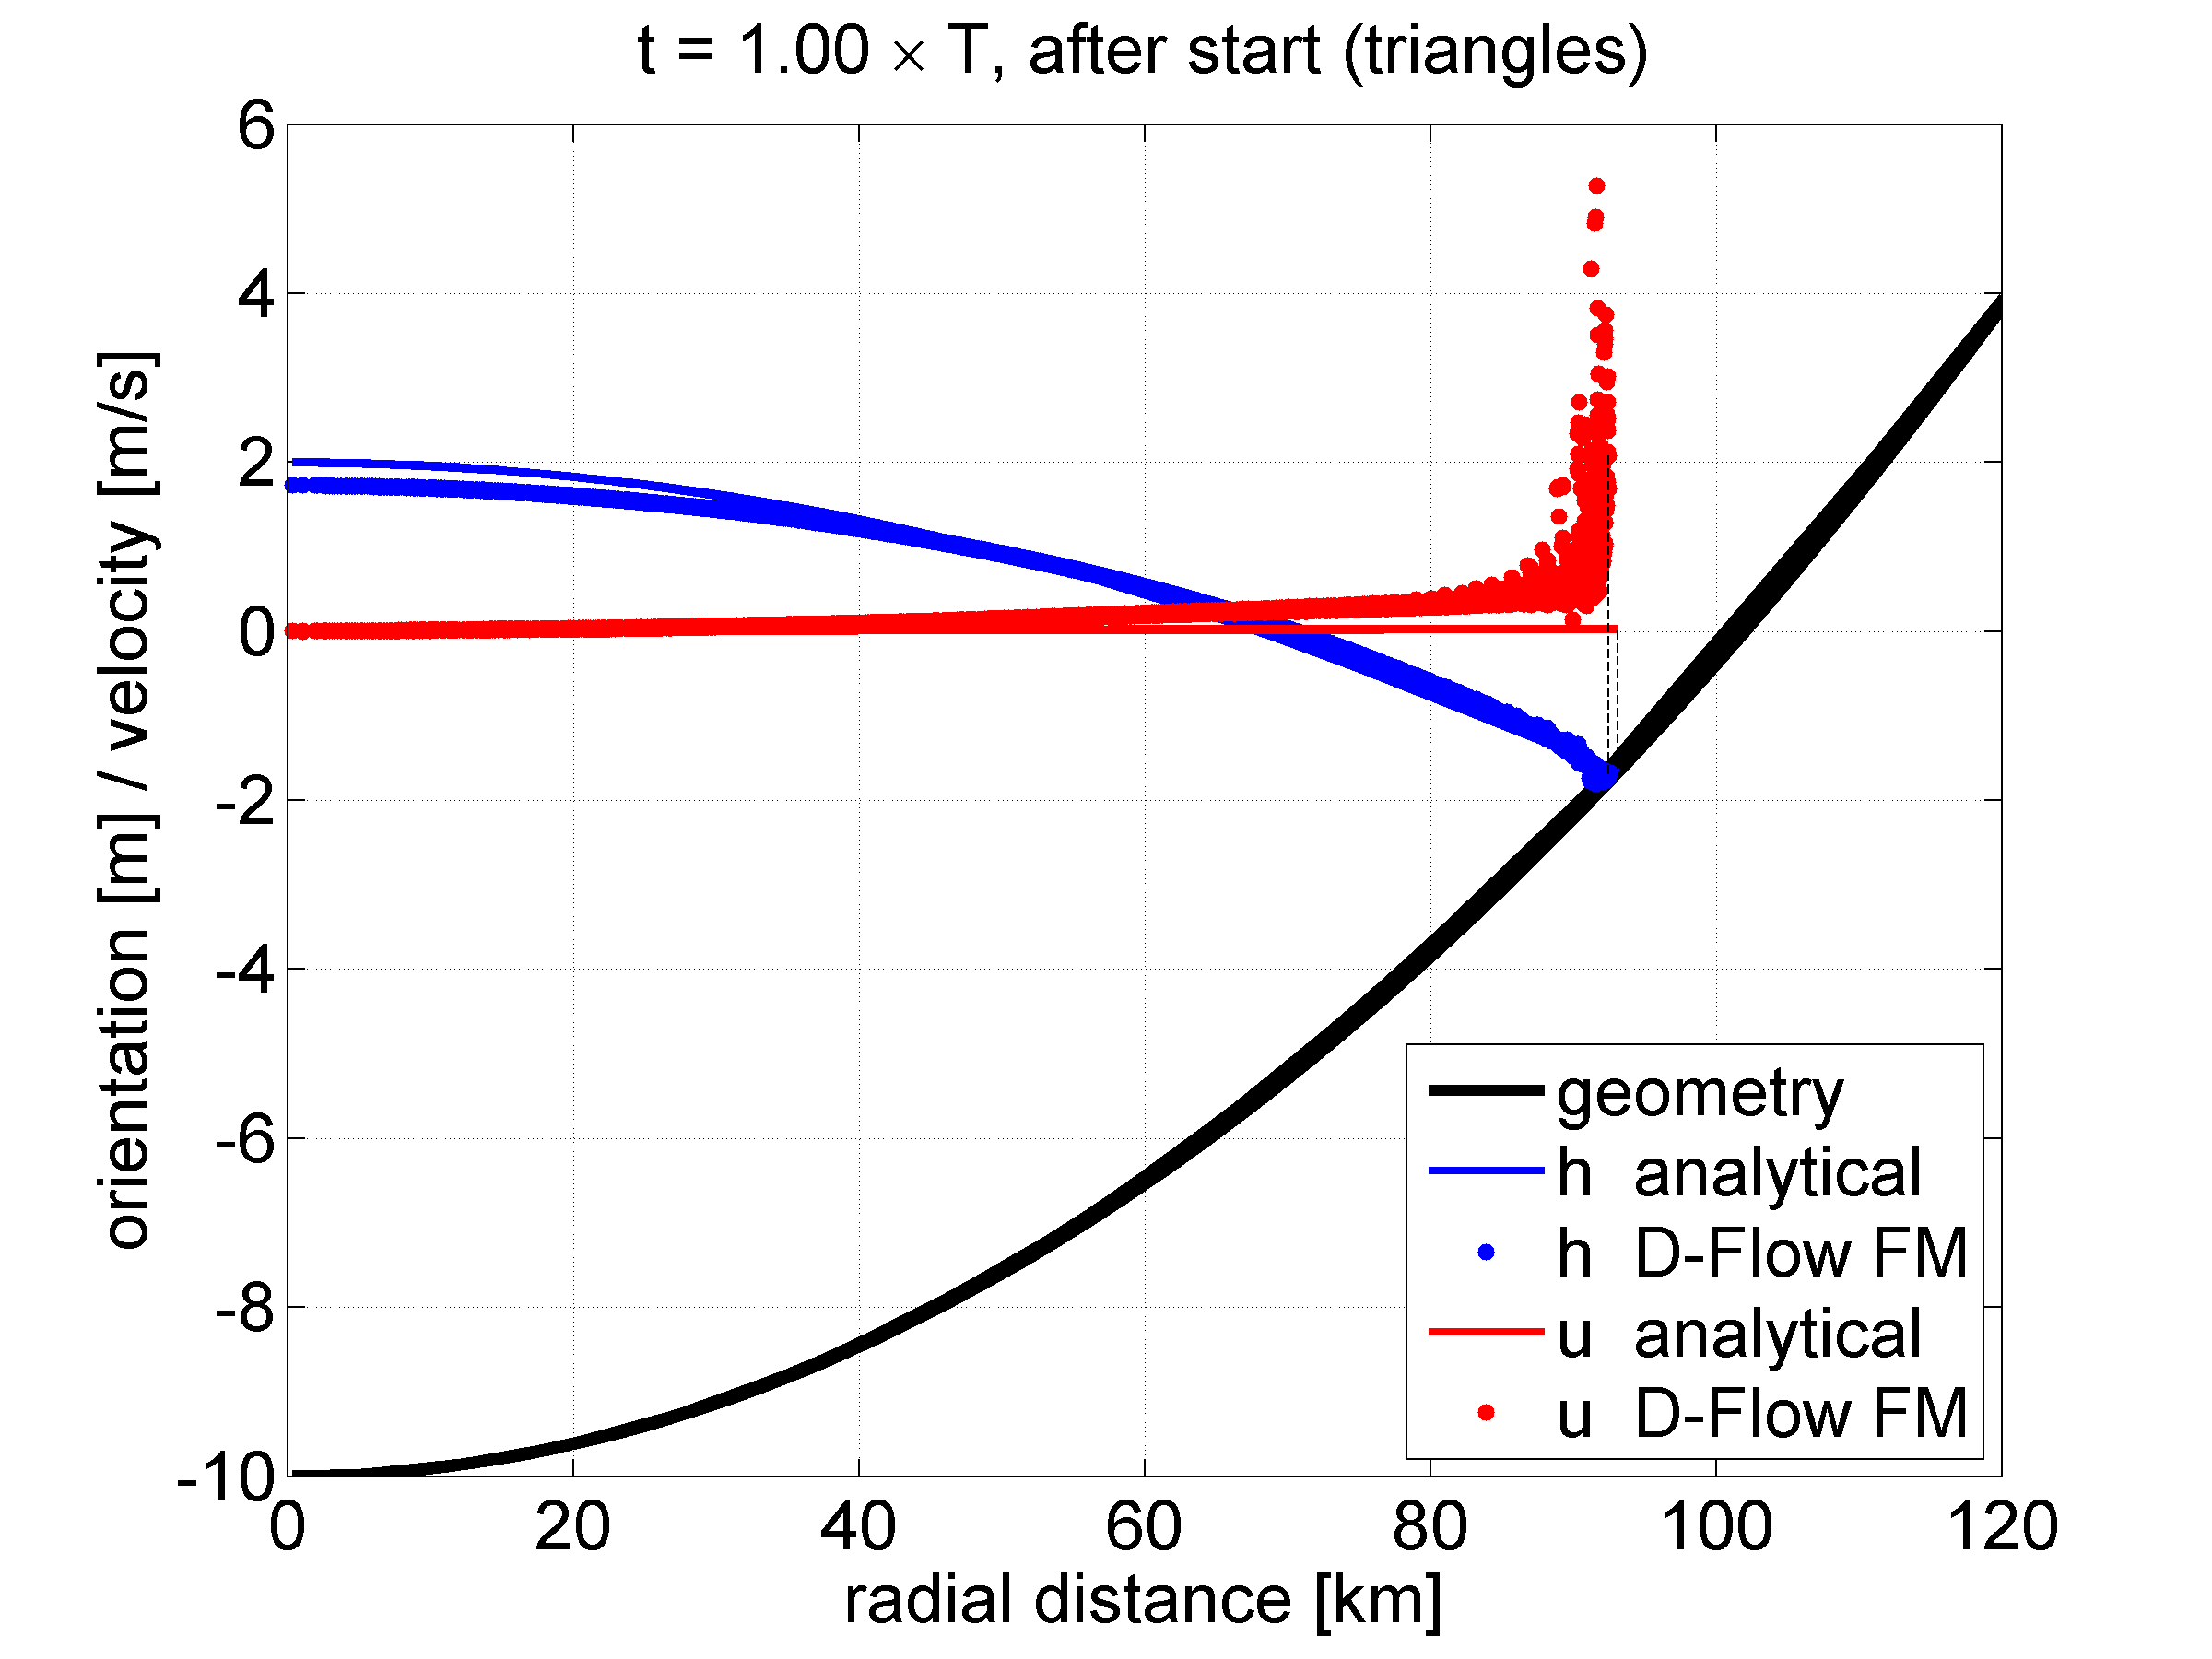
\includegraphics[width=0.48\columnwidth]{../../c045_thacker2d_triangles/doc/figures/thacker2dtrianglesT1.png}
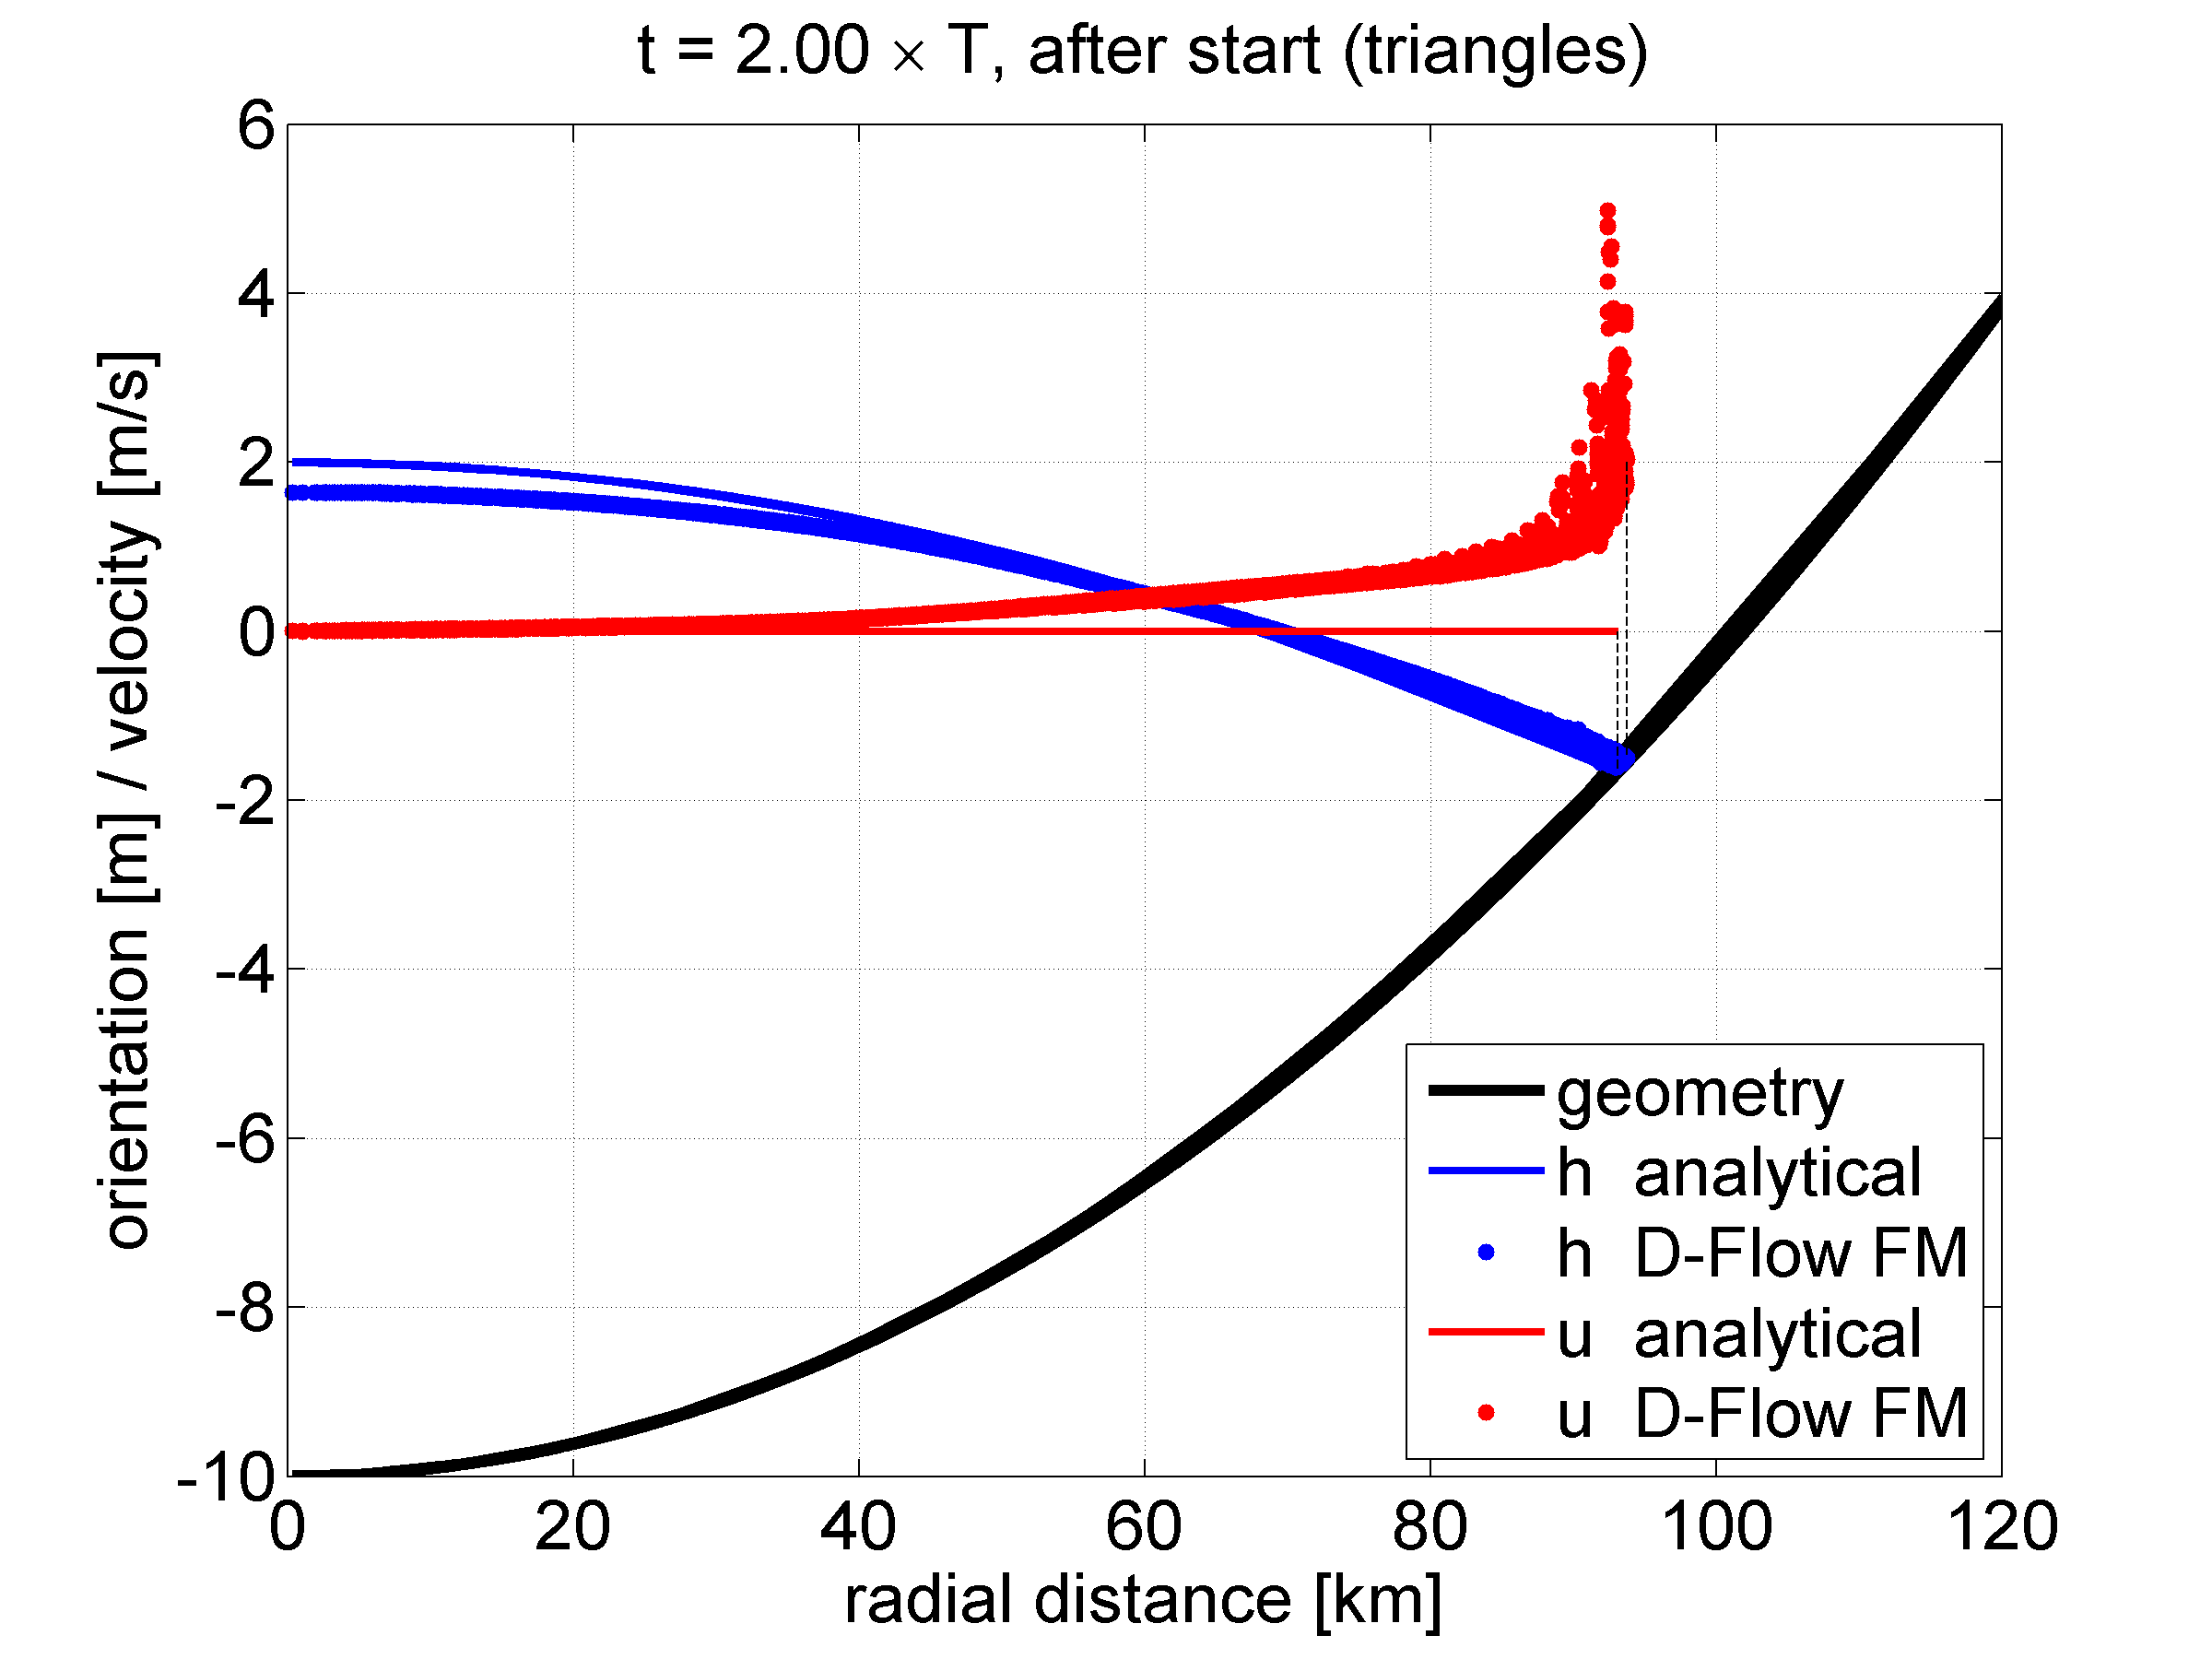
\includegraphics[width=0.48\columnwidth]{../../c045_thacker2d_triangles/doc/figures/thacker2dtrianglesT2.png}
\end{center}\caption{Computational results for the testcase on the hexagonal grid (upper panels), square grid (center panels) and triangular grid (bottom panels) after one period cycle (left panels) and after two period cycles (right panels). \label{fig:thacker2dresults}}
\end{figure}

It is relevant to notice that the three grids, shown in \Fref{fig:thacker2dgrids}, contain cells of different size. The grid containing hexagons is the coarsest, the triangular grid is the finest. This different grade of refinement is also reflected in the numerical results: the top panels in \Fref{fig:thacker2dresults} reveal the largest deviations from the analytical solution, whereas the bottom panels show the smallest deviations from the analytical solution.

A remarkable aspect of the output results is the presence of relatively high velocities near the shoreline. These high velocities appear particularly during drying. For the triangular grid (bottom panels in \Fref{fig:thacker2dresults}), these high velocities are accompanied with quite some scatter, which suggests that the output results are not perfectly radialsymmetric.




\paragraph*{Conclusion}
\DFLOWFM is able to computationally deal with flooding and drying in two-dimensional model configurations. For a relatively coarse grid, considerable deviations are accounted. In the shoreline area, considerable velocities are computed which are likely to be due to relative small water depths.



\paragraph*{Version}
This test has been carried out with version dflow-fm-x64-1.1.132.38471.


